\documentclass[10pt]{beamer}
\usetheme{Frankfurt}
\mode<presentation>
\usepackage[]{xcolor}
\usepackage{minted}
\usepackage{listings}
\usepackage{multicol}
\usepackage{amsmath}
\usepackage{tikz}
\usepackage[most]{tcolorbox}
\usepackage{textpos}
\usepackage{tabularx}
\usepackage{multirow}
\usepackage{multicol}
\usepackage{amsmath}
\usepackage{pdfpages}
\usepackage{verbatim}
\usepackage{float}
\usepackage{changepage}
\usepackage[export]{adjustbox}
%\setbeamertemplate{background}{
%	\tikz[overlay,remember picture]
%	\node[opacity=.05]at (current page.center){
\includegraphics[width=0.3\textwidth]{nec-logo}};
%}
\newcommand{\widthofbold}[1]{%
	\settowidth{\dimen0}{\textbf{#1}}%
\makebox[\dimen0]{#1}}
\newcommand<>{\myword}[1]{%
\alt#2{\textbf{#1}}{\widthofbold{#1}}}
\addtobeamertemplate{frametitle}{}{%
	\begin{textblock*}{70mm}(.935\textwidth,-0.75cm)
		
\includegraphics[height=0.65cm]{nec-logo}
\end{textblock*}}
\newminted{python}{fontsize=\scriptsize,
	linenos,
	numbersep=1pt,
	frame=lines,
	bgcolor=bg,
framesep=3mm}
\DeclareMathOperator*{\argmin}{arg\,min}
\DeclareMathOperator*{\argmax}{arg\,max}
\definecolor{rosso}{RGB}{220,57,18}
\definecolor{giallo}{RGB}{255,153,0}
\definecolor{blu}{RGB}{102,140,217}
\definecolor{verde}{RGB}{16,150,24}
\definecolor{viola}{RGB}{153,0,153}

\makeatletter

\tikzset{
	invisible/.style={opacity=0},
	visible on/.style={alt={#1{}{invisible}}},
	alt/.code args={<#1>#2#3}{%
		\alt<#1>{\pgfkeysalso{#2}}{\pgfkeysalso{#3}} % \pgfkeysalso doesn't change the path
	},
}
%remove the icon
\setbeamertemplate{bibliography item}{}

%remove line breaks
\setbeamertemplate{bibliography entry title}{}
\setbeamertemplate{bibliography entry location}{}
\setbeamertemplate{bibliography entry note}{}
\addtobeamertemplate{navigation symbols}{}{ \hspace{1em}    \usebeamerfont{footline}%
\insertframenumber / \inserttotalframenumber }

% defining text colors
\newcommand{\blue}[1]{\textcolor{blue}{#1}}
\newcommand{\red}[1]{\textcolor{red}{#1}}
\newcommand{\orange}[1]{\textcolor{orange}{#1}}
\newcommand{\green}[1]{\textcolor{green}{#1}}
\newcommand{\black}[1]{\textcolor{black}{#1}}
\newcommand{\yellow}[1]{\textcolor{yellow}{#1}}
\newcommand{\white}[1]{\textcolor{white}{#1}}

% define commands for this presentation only
\newcommand{\mydef}[1]{{\textbf{#1}}}
%\newcommand{\mydef}[1]{{\emph{#1}\/}}
\newcommand{\varname}[1]{{\emph{#1}}}


%--------------
% General Flags
% -------------

% Does every process take one input item and generates one output item?
\newcommand{\singleInSingleOut}[2]{#1}

% Enable CFP mechanism?
\newcommand{\withcfp}[2]{#2}

% Force signature. If true, (#1), then no calls to sign_contract or sign_all_contracts will be run and all agreements (concluded contracts) are immediately binding
\newcommand{\forcesignature}[2]{#2}

% True if we have zero signing delay.
\newcommand{\zerosigndelay}[2]{#1}

% Batch signature. If true, (#1), then the agent is asked to sign ALL contracts concluded at one step together instead of being asked to sign them one by one.
\newcommand{\batchsignature}[2]{#1}

% Keeps a running trading price for each product.
\newcommand{\tradingprice}[2]{#1}

%---------------------------------------
% Breach processing and bankruptcy flags
% --------------------------------------

% Can the agent borrow money (i.e. can its balance go negative)? If False (#2), agents will go bankrupt immediately when their balance hits zero. If true, agents will go bankrupt when their balance hits -bankruptcy_limit and they will be paying interest_rate interest per step for any negative balance (combined interest)
\newcommand{\canborrow}[2]{#2}

% Enable borrowing? If enabled, it allows the balance to go to negative values during breach resolution. money breaches, inventory breaches, and failure to pay penalties all will lead to forced borrowing if this is enabled.
\newcommand{\forceborrow}[2]{#2}

% Enables an external spot market that is used to buy missing products in cases product breaches.
\newcommand{\forcespot}[2]{#1}

% Allows agents committing breaches (product/money) to run immediate fast negotiations with any partners to (buy/sell) products to cover the breach.
\newcommand{\spotnegotiations}[2]{#2}

% Report breaches even after borrowing to pay for them? No matter what is the setting here, a breach will be reported if borrowing did not resolve the issue. This flag takes effect only if the breach was not resolved through borrowing.
\newcommand{\reportbreach}[2]{#1}

% Global breach penalty paid to ``society''
\newcommand{\breachpenalty}[2]{#2}

% Proportional partial execution for contracts at the same time-step. If False, execution is at a predefined order for contracts with the same delivery time.
\newcommand{\proportionalCompensation}[2]{#2}

% Order contracts with the same delivery time by the singing time during bankruptcy processing
\newcommand{\orderBySigningTime}[2]{#1}

%----------------------------------
% External Contract Execution flags
% ---------------------------------

% IF true, exogenous contracts are treated exactly like normal contracts
\newcommand{\externalLikeNormal}[2]{#1}

% The external contracts are only known up to some future horizon (the other option is that they are known for the whole length of the simulation)?
\newcommand{\withhorizon}[2]{#1}

% Force external contracts to be executed in full (the other option is to allow the agent to choose the quantity it wants to execute)?
\newcommand{\forceexternal}[2]{#1}

% Whether to allow agents to borrow for external contracts
\newcommand{\externalBorrow}[2]{#1}
% Whether to allow agents to go bankrupt for external contracts
\newcommand{\externalBankrupt}[2]{#1}

%--------------------------------
% Production flags (Factory step)
% -------------------------------

% Whether to allow agents to borrow for external contracts
\newcommand{\productionBorrow}[2]{#1}
% Whether to allow agents to go bankrupt for external contracts
\newcommand{\productionBankrupt}[2]{#1}
% If true, production failures are silent. Otherwise, production can lead to borrowing to execute it. If \canborrow is false, this MUST be true.
\newcommand{\silentfailure}[2]{#1}

%----------------
% Other commands
% ---------------


\newcommand{\external}{exogenous}
\newcommand{\External}{Exogenous}
\newcommand{\transaction}{contract}
\newcommand{\Transaction}{Contract}
\newcommand{\TimeHorizon}{T}
\newcommand{\SetOfContracts}{C}
\newcommand{\Contract}{c}
\newcommand{\moneyunit}{dollar}
\newcommand{\moneyunits}{dollars}
\newcommand{\CFP}{\text{CFP}}
\newcommand{\Raw}{\text{Raw}}
\newcommand{\Final}{\text{Final}}
\newcommand{\Intermediate}{\text{Intermediate}}
\newcommand{\In}{\text{In}}
\newcommand{\Out}{\text{Out}}
\newcommand{\inn}{\text{in}}
\newcommand{\out}{\text{out}}
\newcommand{\buy}{\text{buy}}
\newcommand{\sell}{\text{sell}}
\newcommand{\yes}{\text{yes}}
\newcommand{\no}{\text{no}}
\newcommand{\tp}{\text{tp}}
\newcommand{\sm}{\text{ip}}
\newcommand{\gl}{\text{gp}}
\newcommand{\cat}{\text{cat}}
\newcommand{\negotiate}{\text{neg}}
\newcommand{\Arg}[1]{{\emph{\hbox{#1}}}}

\newcommand{\credit}{\text{cr}}
\newcommand{\cv}{\text{cv}}
\newcommand{\MABL}{\text{MABL}}
\newcommand{\BrReNeg}{\text{BrReNeg}}
\newcommand{\BrPen}{\text{BrPen}}
\newcommand{\ReNegBrPen}{\text{ReNegBrPen}}
\newcommand{\nf}{n^f}
\newcommand{\Uniform}[2]{\ensuremath{\mathcal{U}\left\{#1, #2\right\}}}
\newcommand{\Normal}[2]{\ensuremath{\mathcal{N}\left\{\mu=#1, \sigma=#2\right\}}}

\newcommand{\level}{l}
\newcommand{\process}{\level}
\newcommand{\product}{p}
\newcommand{\factory}{f}
\newcommand{\agent}{\factory}
\newcommand{\nProcesses}{L}
\newcommand{\nLevels}{\nProcesses}
\newcommand{\nProducts}{P}
\newcommand{\nFactories}{F}
\newcommand{\nFactoriesPerLevel}{F_\level}
\newcommand{\nFactoriesGeneratingProduct}{F_{\product-1}}
\newcommand{\cost}{c}
\newcommand{\costPerProcess}{c_\process}
\newcommand{\costPerFactory}{c_\factory}
\newcommand{\step}{d}
\newcommand{\profit}{\pi}
\newcommand{\productivity}{\eta}
\newcommand{\cashAvailability}{a}
\newcommand{\exgenousControllability}{e}
\newcommand{\catalogPrice}{g}
\newcommand{\activeLines}{A}
\newcommand{\quantityProducible}{Q}
\newcommand{\exogenoutQuantity}{q}
\newcommand{\nExogenous}{n}
\newcommand{\nCompetitors}{C}
\newcommand{\competitor}{i}
\newcommand{\nAgentsPerCompetitor}{A_\competitor}
\newcommand{\CompetitorList}{\mathcal{C}}
%\newcommand{\CompetitorList}{\{ 0, \ldots, \nCompetitors-1 \}}
\newcommand{\balance}{b}
\newcommand{\nRepetition}{K}
\newcommand{\nCompetitorsPerWorld}{M}
\newcommand{\nSteps}{S}
\newcommand{\nLines}{\nu}

\newtheorem{remark}{Remark}

\begin{document}
\title{Automated Negotiation}
\subtitle{A Tutorial}
\author{\textbf{Yasser Mohammad}$^{1,2}$}
\institute{$^1$ NEC-AIST Collaborative Lab., AIST, Japan \and $^2$ Assiut University, Egypt}
\date{October 29, 2019}

\begin{frame}
	\titlepage
\end{frame}
\begin{frame}
	\frametitle{Outline}
	\tableofcontents[pausesections,hideallsubsections]
	%\tableofcontents
\end{frame}
\AtBeginSection[]
{
	\begin{frame}[shrink]
		\frametitle{Outline}
		\tableofcontents[currentsection,currentsubsection,subsectionstyle=show/show/hide]
		%\tableofcontents[sectionstyle=show/hide,subsectionstyle=hide/show/hide]
	\end{frame}
	\addtocounter{framenumber}{-1}
}
\AtBeginSubsection[]
{
	\begin{frame}[shrink]
		\frametitle{Outline}
		\tableofcontents[currentsection,currentsubsection,subsectionstyle=show/shaded/hide]
		%\tableofcontents[sectionstyle=show/hide,subsectionstyle=hide/show/hide]
	\end{frame}
	\addtocounter{framenumber}{-1}
}

\section[Negotiation]{Negotiation}
\begin{frame}[label=neg]
	\centering
	\includegraphics<1>[page=1,width=.75\textwidth]{figs/overview.pdf}
	\includegraphics<2>[page=2,width=.75\textwidth]{figs/overview.pdf}
	\includegraphics<3>[page=3,width=.75\textwidth]{figs/overview.pdf}
	\includegraphics<4>[page=4,width=.75\textwidth]{figs/overview.pdf}
	\includegraphics<5->[page=5,width=.75\textwidth]{figs/overview.pdf}
	\setbeamercovered{transparent}
	\begin{itemize}
		\item<6-> A method to achieve agreement among self-interested actors.
		\item<7-> Negotiation is important  $\rightarrow$ win-win agreements.
		\item<8-> Automatic Negotiation $\rightarrow$ $\$\$\$$
			\begin{itemize}
				\item smart contracts, resource allocation, SCM, etc
			\end{itemize}
	\end{itemize}
\end{frame}

% \begin{frame}{Definition}
% 	\begin{block}{Negotiation}
% 		$\varUpsilon \equiv \left(A, T, N,\Omega, M, \left\{\tilde P_a, P^n_{ab} \text{ }\forall 1 \le a, b \le A,\text{  }0\le n\le N \right\}\right)$
%
% 		\begin{description}
% 			\pause
% 		\item[$A \in \mathbf{I^+} - \left\{1\right\}$:] Number of agents/actors. \pause
% 		\item[$T \in \mathbf{R} \bigcup \infty $:] The allowed time of the negotiation. \pause
% 		\item[$N \in \mathbf{I} \bigcup \infty$:] The allowed number of rounds of the negotiation. \pause
% 		\item[$\Omega \equiv \left\{\omega_j\right\} \bigcup \phi$:] Possible outcomes including $\phi$ signifying disagreement. \pause
% 		\item[$M$] The negotiation \emph{mechanism} (protocol) defining rules of encounter for agents. \pause
% 		\item[$\tilde{P}_{a}$:] Preferences of \textbf{actor} $a$. \pause
% 		\item[${P}_{ab}^n$:] Information available to \textbf{agent} $a$ about preferences of \textbf{actor} $b$ at the beginning of round $n$.
% 	\end{description}
% \end{block}
%
% \pause
% \begin{alertblock}{Known Preferences Assumption}
% 	$P^n_{aa}  = \tilde P_a$
% \end{alertblock}
% \end{frame}
%
% \begin{frame}{Preference Representations}
% 	\begin{block}{Preference Types}
% 		\begin{description}
% 			\item[Partial Ordering $\succcurlyeq$] Defines preference as a partial ordering over $\Omega$.
% 			\item[Ranking] A total ordering over a subset of $\Omega$.
% 			\item[Utility Function $\tilde u$] Defines a numeric value for every outcome in $\Omega$.
% 				\[\tilde{u}: \Omega \rightarrow \Re\]
% 			\item[Probabilistic Utility Function $u$] Defines a distribution of values.
% 				\[{u}: \Omega \times \Re \rightarrow  [0, 1{]}\]
% 		\end{description}
% 	\end{block}
% 	\begin{alertblock}{Known Ufun Assumption}
% 		\[u^t_a \left(\omega, x\right) = u^0_a \left(\omega, x\right) = \begin{cases}
% 			1 & \tilde u\left(\omega\right) = x\\
% 			0 & otherwise
% 		\end{cases}\]
% 	\end{alertblock}
% \end{frame}
\begin{frame}{Components of the Negotiation Problem}
	\centering
	\includegraphics[page=4,width=0.5\textwidth]{figs/overview.pdf}
	\begin{description}
		\item[Negotiation Protocol] Defines how negotiation is to be conducted [Mechanism Design Problem].
			\begin{itemize}
				\item Alternating Offers Protocol
				\item Single Text Protocol
				\item \dots
			\end{itemize}
		\item[Negotiation Strategy] Defines how an agent behaves during the negotiation [Effective Negotiation Problem].
			\begin{itemize}
				\item Time-based strategies: Boulware, conceder, \dots
				\item Tit-for-tat variations
				\item \dots
			\end{itemize}
	\end{description}
\end{frame}
\begin{frame}{Important Concepts}
	\centering
	\tcbox[width=1\textwidth]{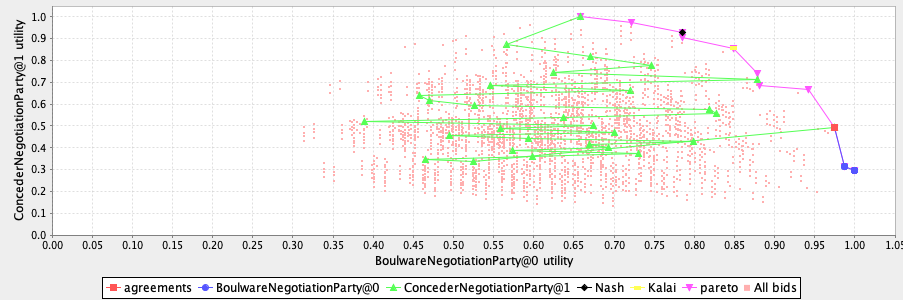
\includegraphics[width=0.8\textwidth]{figs/session.png}}

	\begin{description}
		\item[Pareto Frontier] Outcomes that cannot be improved for one actor without making another worse off.
		\item[Welfare] Total utility received by all actors.
		\item[Surplus utility] Utility above disagreement utility.
	\end{description}
\end{frame}

\begin{frame}{Types of Automated Negotiation Problems}
	\begin{columns}
		\begin{column}{0.5\textwidth}
			\begin{block}<2->{Negotiator type}
				\begin{enumerate}
					\item Agent-Agent negotiation
					\item Agent-Human negotiation
				\end{enumerate}
			\end{block}

			\begin{block}<3->{Number of negotiators}
				\begin{enumerate}
					\item Bilateral negotiation
					\item Multilateral negotiation
				\end{enumerate}
			\end{block}

			\begin{block}<4->{Outcome Space}
				\begin{enumerate}
					\item Single Issue: $\Omega=\left\{\omega_0, \omega_1, ....\right\}$
					\item Multiple Issues: $\Omega=\prod_{i=1}^{n_i}I_i$
				\end{enumerate}
			\end{block}
			\begin{block}<5->{Protocol Type}
				\begin{enumerate}
					\item Mediated
					\item Unmediated
				\end{enumerate}
			\end{block}
		\end{column}
		\begin{column}{0.5\textwidth}
			\tcbox[colback=white]{\includegraphics[page=5,width=0.8\textwidth]{figs/overview.pdf}}

		\end{column}
	\end{columns}
\end{frame}

% \begin{frame}{Platforms [Used in this tutorial]}
% 	\begin{block}{Genius \cite{Genius}}
% 		\begin{columns}
% 			\begin{column}{0.65\textwidth}
% 				a Java-based negotiation platform to develop general negotiating agents and create negotiation scenarios. The platform can simulate negotiation sessions and tournaments and provides analytical tools to evaluate the agents' performance.
% 			\end{column}
% 			\begin{column}{0.2\textwidth}
% 				
\includegraphics[width=\columnwidth]{figs/Genius_logo.png}
% 			\end{column}
% 		\end{columns}
% 	\end{block}
% 	\begin{block}{NegMAS \cite{negmas}}
% 		\begin{columns}
% 			\begin{column}{0.65\textwidth}
% 				a Python-based negotiation platform for developing autonomous negotiation agents embedded in simulation environments.The main goal of NegMAS is to advance the state of the art in situated simultaneous negotiations.
% 			\end{column}
% 			\begin{column}{0.2\textwidth}
% 				
\includegraphics[width=\textwidth]{figs/negmas.png}
% 			\end{column}
% 		\end{columns}
%
% 	\end{block}
% \end{frame}

\subsection[SAOP]{Unmediated Protocols}

\begin{frame}{Unmediated Protocols}
	\begin{block}{Main Features}
		\begin{columns}
			\begin{column}{.6\textwidth}
				\begin{itemize}
					\item No central coordinator.
					\item Agents negotiate by exchanging \emph{messages}.
					\item All proposals come from negotiators.
				\end{itemize}
			\end{column}
			\begin{column}{.4\textwidth}
				\tcbox[colback=white]{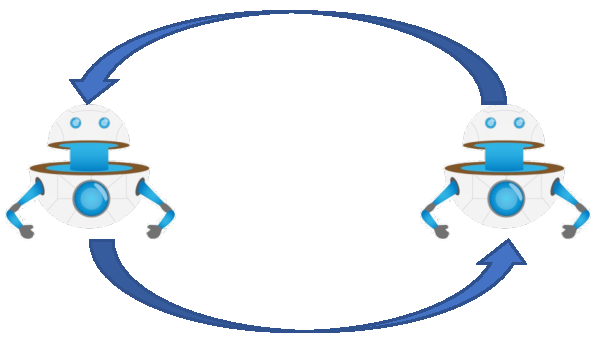
\includegraphics[width=.6\columnwidth]{figs/unmediated}}
			\end{column}
		\end{columns}
	\end{block}
	\pause
	\begin{block}{Examples}
		\begin{description}
			\item [Nash Bargaining Game] Single iteration, single issue, bilateral protocol with complete information.
			\item [Rubinstein Bargaining Protocol] Infinite horizon, single issue, bilateral protocol with complete information \cite{rubinstein1982perfect}.
			\item [Stacked Alternating Offers Protocol] Finite horizon, multi-issue, multilateral protocol with partial information \cite{aydougan2017alternating}.
		\end{description}
	\end{block}
\end{frame}

\subsection[Bargaining]{The Simplest Negotiation}

\begin{frame}{Nash Bargaining Game: Description}
	\begin{columns}
		\begin{column}{0.6\textwidth}
			A single-step full-information bilateral negotiation with $\Omega = [0, 1]^2$ and two utility functions ($\tilde u_1, \tilde u_2$) such that:
			\begin{itemize}
				\item<2-> A (usually convex) feasible set of agreements $F$. A common example is to define $F$ as all the outcomes for which
					the total utility received by negotiators is less than or equal to one:
					\[F = \left\{(\omega_1, \omega_2) | \tilde u_2(\omega_2) + \tilde u_1(\omega_1) \le 1\right\}.\]
				\item<5-> A disagreement point $d \equiv  \tilde u_1(\phi) + \tilde u_2(\phi) \in \Re^2$ which is the utility value received by the two players in case of disagreement (
					reserved values).
			\end{itemize}
		\end{column}
		\begin{column}{0.4\textwidth}
			\def\angle{0}
			\def\radius{3}
			\def\cyclelist{{"red","blue","gray"}}
			\newcount\cyclecount \cyclecount=-1
			\newcount\ind \ind=-1
			\resizebox{0.8\columnwidth}{!}{%
				\begin{tikzpicture}[nodes = {font=\sffamily}]
					\foreach \percent/\name in {
						30/First Agent,
						50/Second Agent,
						20/Lost
						} {
						\ifx\percent\empty\else               % If \percent is empty, do nothing
							\global\advance\cyclecount by 1     % Advance cyclecount
							\global\advance\ind by 1            % Advance list index
							\ifnum3<\cyclecount                 % If cyclecount is larger than list
								\global\cyclecount=0              %   reset cyclecount and
								\global\ind=0                     %   reset list index
							\fi
							\pgfmathparse{\cyclelist[\the\ind]} % Get color from cycle list
							\edef\color{\pgfmathresult}         %   and store as \color
							% Draw angle and set labels
							\draw[fill={\color!50},draw={\color}] (0,0) -- (\angle:\radius)
								arc (\angle:\angle+\percent*3.6:\radius) -- cycle;
							\node at (\angle+0.5*\percent*3.6:0.7*\radius) {\percent\,\%};
							\node[pin=\angle+0.5*\percent*3.6:\name]
								at (\angle+0.5*\percent*3.6:\radius) {};
							\pgfmathparse{\angle+\percent*3.6}  % Advance angle
							\xdef\angle{\pgfmathresult}         %   and store in \angle
							\fi
						};
				\end{tikzpicture}
			}
			\resizebox{1.0\textwidth}{!}{%
				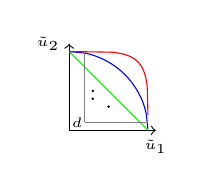
\begin{tikzpicture}
					\draw[->] (0,0) -- (1.1,0) node[anchor=north,visible on=<2->] {\tiny $\tilde u_1$};
					\draw[->] (0,0) -- (0,1.1) node[anchor=east,visible on=<2->] {\tiny $\tilde u_2$};
					\node[circle,fill=black,inner sep=0pt,visible on=<6->] at (0.3, 0.5) {};
					\node[circle,fill=black,inner sep=0pt,visible on=<6->] at (0.5, 0.3) {};
					\node[circle,fill=black,inner sep=0pt,visible on=<6->] at (0.3, 0.4) {};
					\draw[domain=0:1,smooth,variable=\x,green,visible on=<2->] plot ({\x},{(1-\x)});
					\draw[domain=0:1,smooth,variable=\x,blue,visible on=<3-4>] plot ({\x^0.5},{(1-\x)^0.5});
					\draw[domain=0:1,smooth,variable=\x,red,visible on=<4>] plot ({\x^0.2},{(1-\x)^0.2});
					\draw[color=gray,visible on=<5->] (0.2, 1) -- (0.2, 0.1) ;
					\draw[color=gray,visible on=<5->] (1, 0.1) -- (0.2, 0.1);
					\draw[visible on=<5->] (0.1, 0.1) node {\tiny $\scriptscriptstyle d$} 	;
				\end{tikzpicture}
			}
		\end{column}
	\end{columns}
\end{frame}

% \begin{frame}{Nash Bargaining Game: Solution}
% 	\begin{itemize}
% 		\item Nash Point (1950): The point at which the product of surplus utility (above reservation value) of negotiators is maximized
% 			\[\argmax_{\omega_1, \omega_2} \prod_{i=1}^2\left(\tilde u_i(\omega_{i}) - \tilde u_i(\phi)\right)\]
% 			\pause
% 		\item Kalai-Smorodinsky Point (1975): The Pareto outcome with equal ratios of achieved  surplus utility and  maximum feasible surplus utility
% 			\[\argmax_{\omega_1, \omega_2 \in F}\left(\omega_1+\omega_2\right)
% 				\text{ s.t. }
% 				\left(\frac{\tilde u_1(\omega_1)-\tilde u_1(\phi)}{\tilde u_2(\omega_2)-\tilde u_2(\phi)} =
% 					\frac{\max_{v \in F} \left(\tilde u_1(v)\right)-\tilde u_1(\phi)}{\max_{v \in F}
% 			\left(\tilde u_2(v)\right)-\tilde u_2(\phi)}\right)\]
% 			\pause
% 		\item Kalai Point (1977): The Pareto outcome maximizing the utility for the unfortunate player. Defining $P$ as the Pareto front
% 			\[\argmax_{\omega_1, \omega_2 \in P} \min_{i \in \{1,2\}}\left(\tilde u_i(\omega_{i}) - \tilde u_i(\phi)\right)\]
% 	\end{itemize}
% \end{frame}
%
% \begin{frame}{Rubinstein's Bargaining Protocol: Description}
% 	\begin{itemize}
% 		\item Two agents sharing a pie.
% 			\pause
% 		\item Each agent is under a different time-pressure: $\tilde u_i^{t+\Delta}(\omega) < \tilde u_i^{t}(\omega)$. Examples of time-pressure:
% 			\pause
% 			\begin{description}
% 				\item[Exponential] $\tilde u_i^{t+\Delta}(\omega) = \delta_i^{\Delta}u_i^{t}(\omega)$.
% 				\item[Linear] $\tilde u_i^{t+\Delta}(\omega) = u_i^{t}(\omega) - \Delta c_i$
% 			\end{description}
% 			\pause
% 		\item Actor's initial utility is the assigned part of the pie: $\tilde u_i^0=\omega_i$.
% 			\pause
% 		\item Time pressure and utility information are common knowledge.
% 			\pause
% 		\item No externally imposed time-limit.
% 			\pause
% 		\item Zero reservation value: $u^{\tau}_i(\phi) = 0\text{ }\forall \tau$.
% 	\end{itemize}
% 	\pause
% 	\begin{block}{Main Result}
% 		There is a unique \emph{sub-game perfect equilibrium} that requires a single negotiation step in most cases.
% 	\end{block}
% \end{frame}
%
% \begin{frame}{Rubinstein's Bargaining Protocol: Equilibrium}
% 	\begin{block}{Exponential Discounting}
% 		The negotiation ends in \textbf{one step} with the first agent proposing and the second agent accepting \emph{for asymmetric cases}:
% 		\[
% 			\left(\omega^*_1, \omega^*_2\right) = \left(\frac{1-\delta_2}{1-\delta_1\delta_2}, \frac{\delta_2\left(1-\delta_1\right)}{1-\delta_1\delta_2}\right)
% 		\]
% 	\end{block}
% 	\pause
% 	\begin{block}{Linear Discounting}
% 		The negotiation ends in \textbf{one step} with the first agent proposing and the second agent accepting:
%
% 		\[
% 			\left(\omega^*_1, \omega^*_2\right) = \begin{cases}
% 				(c_2, 1- c_2)	& c_1 > c_2\\
% 				(x, 1-x)\text{ }\forall x \in [c_1, 1]	& c_1 = c_2\\
% 				(1, 0)	& c_1 < c_2\\
% 			\end{cases}
% 		\]
%
% 	\end{block}
%
% \end{frame}

% \section[Strategies]{Strategies for SAOP}
%
% \begin{frame}[fragile]
% 	\frametitle{Stacked Alternating Offers Protocol}
% 	\begin{minted}[linenos=true]{python}
% 			n_agreed, current = 0, randint(0, n_agents)
% 			offer = agents[current].offer()
% 	\end{minted}
% 	\pause\vspace{-2pt}
% 	\begin{minted}[linenos=true]{python}
% 			while True:
% 			if timedout():
% 			return 'TIME_OUT'
% 			current = (current + 1) % n_agents
% 			response = agents[current].respond(offer)
% 			if response == 'accept':
% 			n_agreed += 1
% 			if n_agreed == n_agents:
% 			return offer  # contract
% 			elif response == 'end_negotiation':
% 			return 'FAILURE'
% 			elif response == 'reject':
% 			offer = agents[current].offer()
% 	\end{minted}
% \end{frame}
%
% \begin{frame}{Negotiator Components \cite{Baarslag2014}\footnote{Supported by Genius}}
% 	\centering
% 	\tcbox{
% 		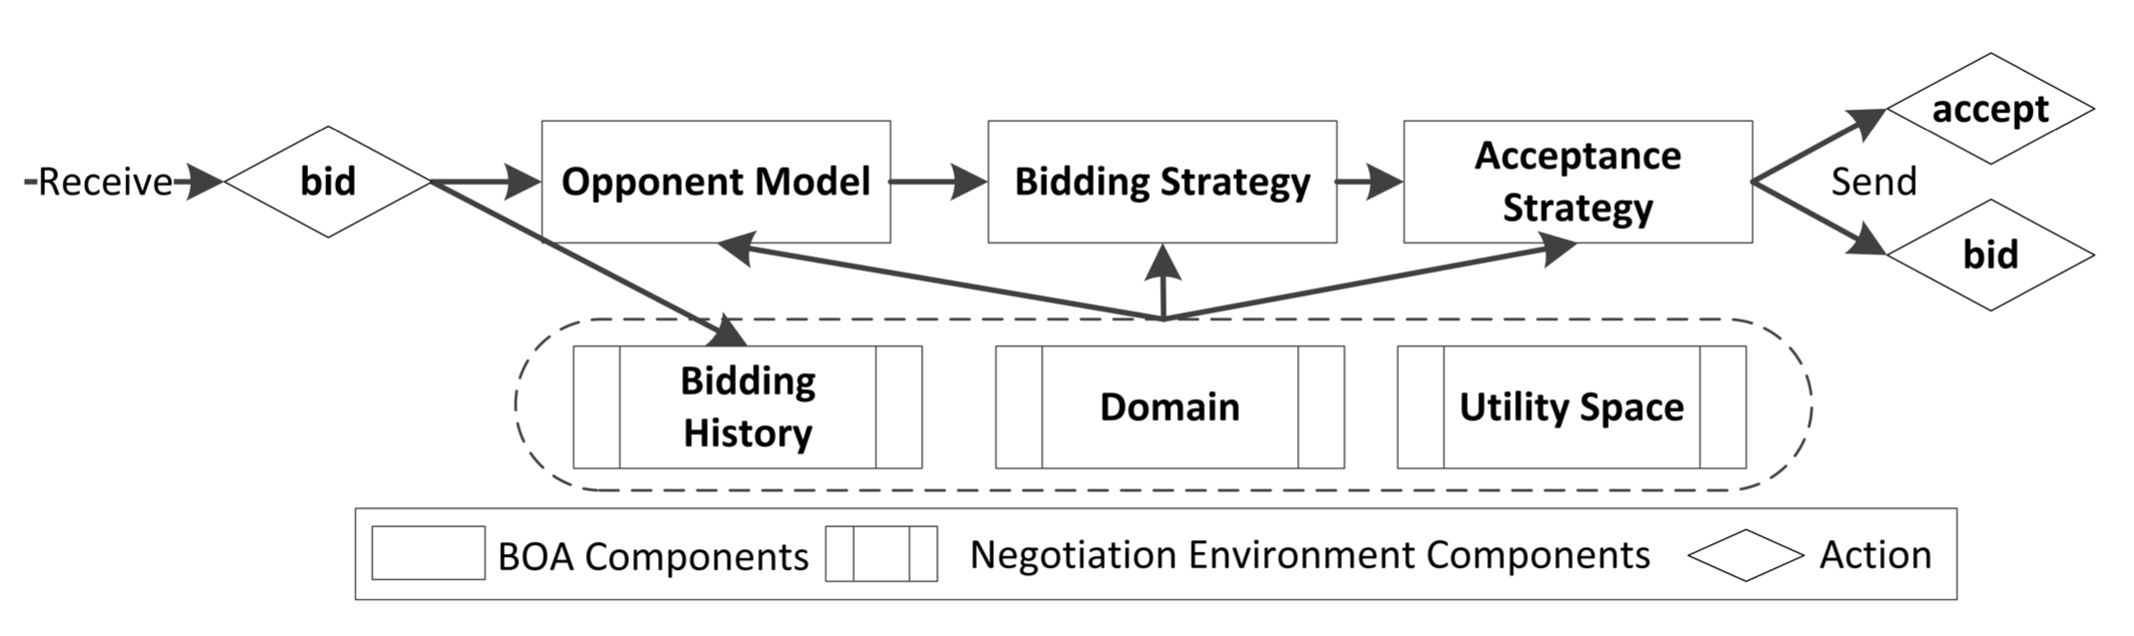
\includegraphics[width=0.9\textwidth]{figs/oba.png}
% 	}
% 	\begin{block}{OBA Atchitecture}
% 		\begin{description}
% 			\item[Opponent Model] predicts opponent behavior.
% 			\item[Bidding Strategy] Generates new bids.
% 			\item[Acceptance Strategy] Decides when to accept.
% 		\end{description}
% 	\end{block}
% \end{frame}
%
% \begin{frame}{Bidding Strategy}
% 	\begin{block}{Time-based strategies}
% 		\begin{columns}
% 			\begin{column}{0.45\textwidth}
% 				Offer an outcome with a utility just above the current \emph{aspiration level} which is monotonically decreasing.
% 			\end{column}
% 			\begin{column}{0.35\textwidth}
% 				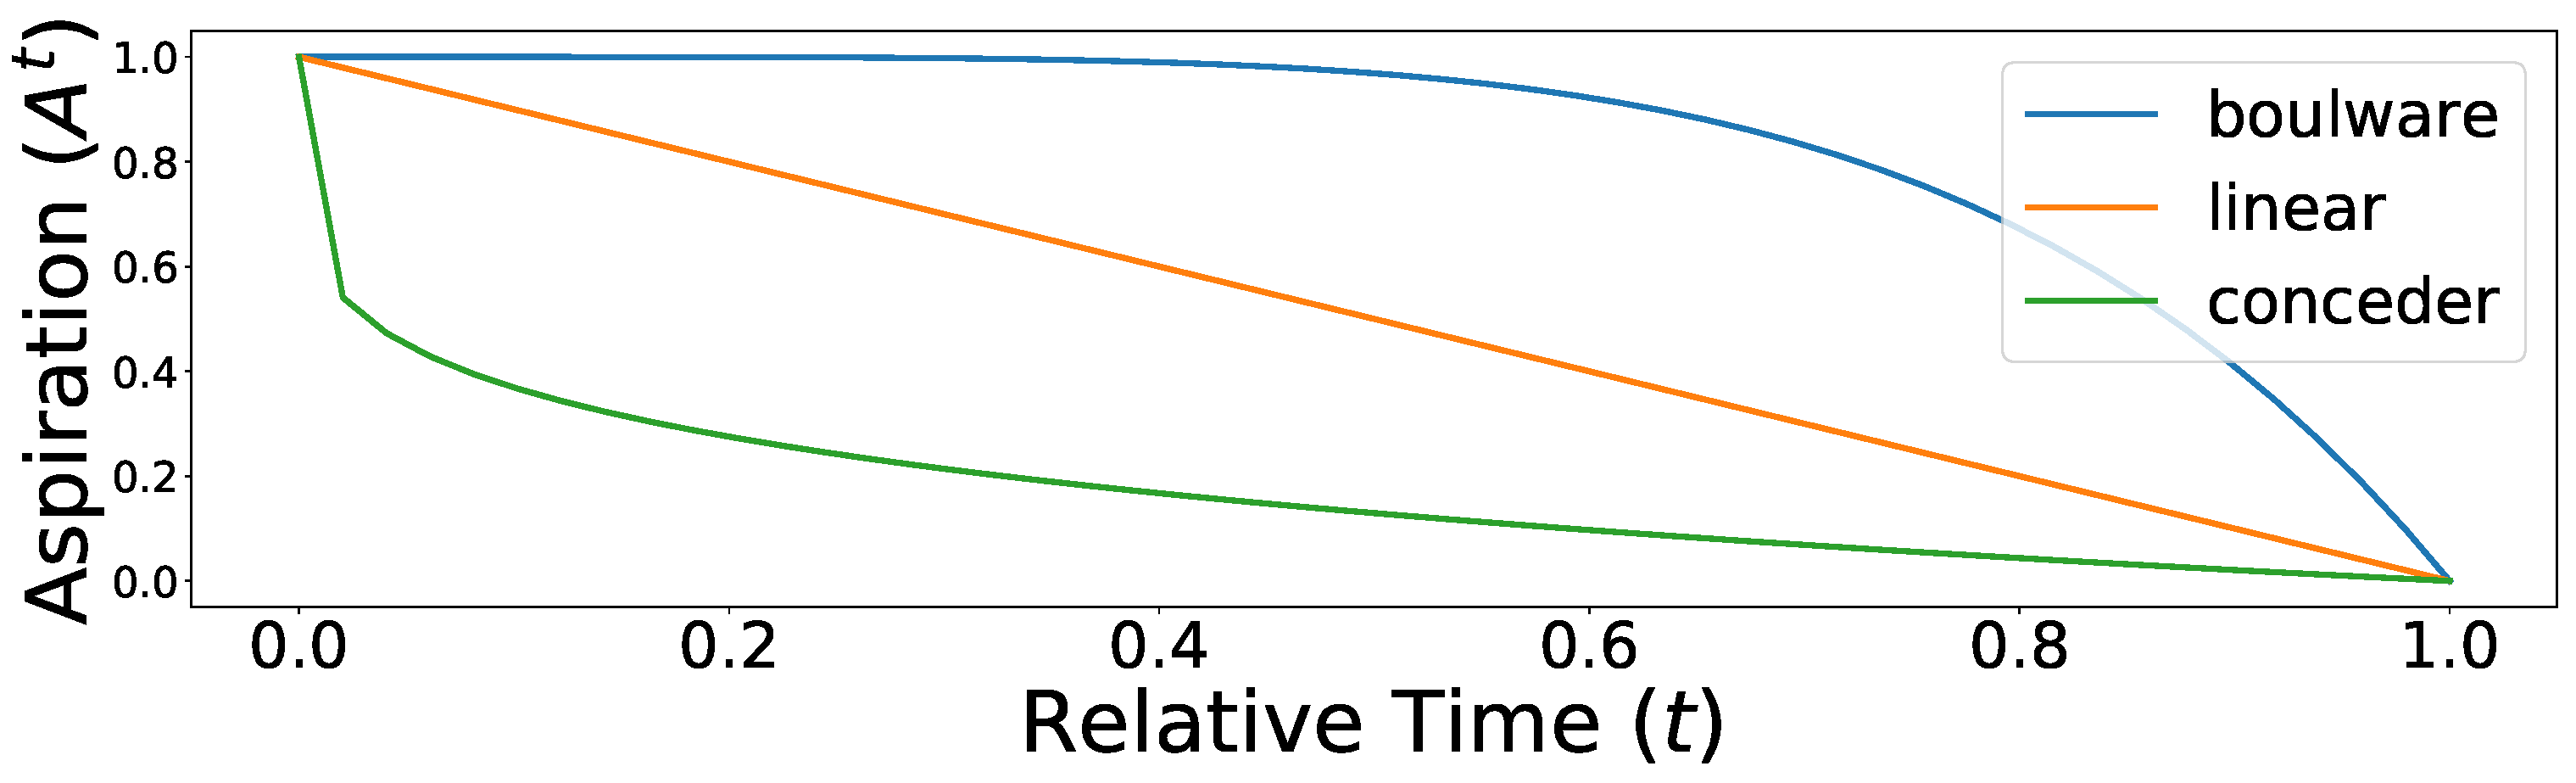
\includegraphics[width=\columnwidth]{figs/aspiration}
% 			\end{column}
% 		\end{columns}
% 	\end{block}
% 	\pause
% 	\begin{block}{(Nice) Tit-for-Tat (bilateral) \cite{baarslag2013tit}}
% 		\begin{columns}
% 			\begin{column}{0.25\textwidth}
% 				Concede as much as the opponent and do not retaliate.
% 			\end{column}
% 			\begin{column}{0.5\textwidth}
% 				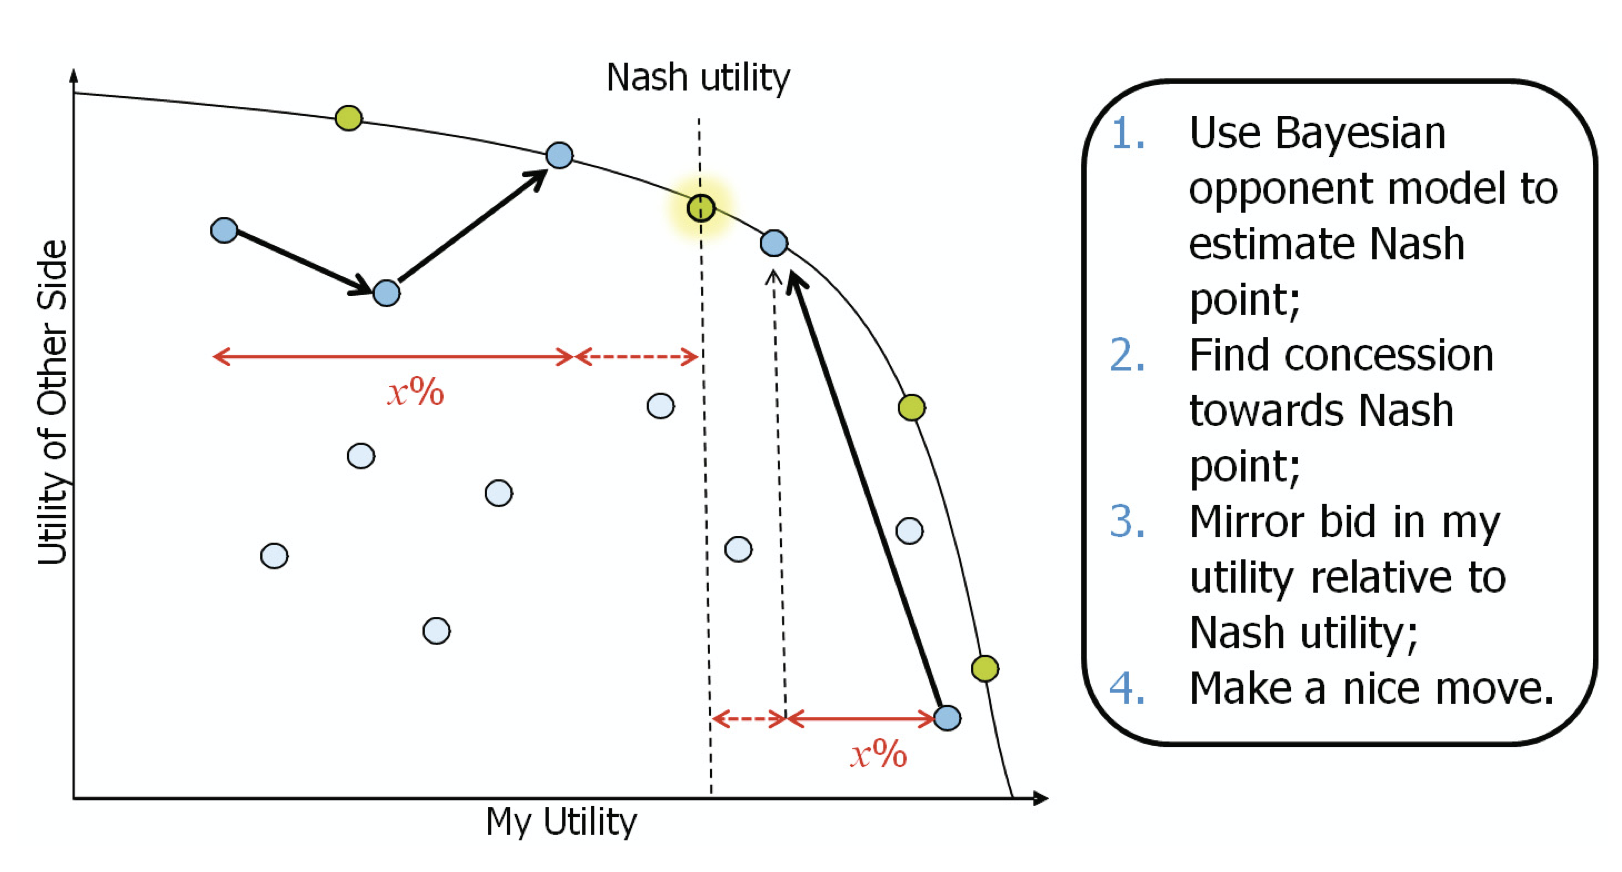
\includegraphics[width=\columnwidth]{figs/nice-tit-for-tat.png}
% 			\end{column}
% 		\end{columns}
% 	\end{block}
% \end{frame}
%
% \begin{frame}{Opponent Modeling}
% 	\begin{block}{What is being modeled?}
% 		\begin{itemize}
% 			\item Opponent preferences.
% 			\item Opponent strategy.
% 			\item Acceptance probability.
% 			\item Future offers.
% 			\item Opponent Type.
% 		\end{itemize}
% 	\end{block}
% 	\pause
% 	\begin{block}{When is it modeled?}
% 		\begin{itemize}
% 			\item Before the negotiation.
% 			\item During the negotiation.
% 		\end{itemize}
% 	\end{block}
% 	\pause
% 	\begin{block}{Data}
% 		\begin{itemize}
% 			\item This negotiation vs. past negotiations.
% 			\item This opponent vs. this opponent group vs. others.
% 			\item Exchanged offers vs. agreements
% 		\end{itemize}
% 	\end{block}
% \end{frame}
%
% \begin{frame}{Opponent Model: Example}
% 	\begin{block}{Bayesian Learning}
% 		\begin{description}
% 			\item[Hypothesis] A hypothesis about the opponent's behavior.
% 				\pause
% 			\item[Evidence] Behavior of the agent (e.g. its offers/rejections).
% 		\end{description}
% 		\pause
% 		\[
% 			P(H|E) = \frac{P(E|H)P(H)}{P(E)}
% 		\]
% 	\end{block}
% 	\pause
% 	\begin{block}{Example}
% 		\textbf{Hypothesis space}: Utility function as a weighted sum of basis functions
% 		\[
% 			u(\omega) = \sum_{i=1}^{n}{\alpha_i f_i(\omega_i; \sigma_i)}
% 		\]
% 		\pause
% 		\textbf{Evidence}: Rejection and offers (assuming a strategy).
% 	\end{block}
% \end{frame}
%
% \begin{frame}{Acceptance Model}
% 	\begin{block}{Examples}
% 		Accept if the utility of the offer $\succ$
% 		\pause
% 		\begin{description}
% 			\item[Previous] my last offer.
% 				\pause
% 			\item[Current] what I am about to offer.
% 				\pause
% 			\item[Expected] the best offer I expect to receive (needs an opponent model).
% 				\pause
% 			\item[Threshold] an offer with the current utility threshold ($\tau$).
% 				\pause
% 				\begin{description}
% 					\item[Constant] May be a fraction of maximum utility.
% 						\pause
% 					\item[Time-based]  Monotonically decreasing with time.
% 						\pause
% 					\item[Predictive] Predicts the expected/max utility on rejection (e.g. Gaussian Process).
% 				\end{description}
% 		\end{description}
% 	\end{block}
% \end{frame}
%
% \section{SCML's Challenge}

% \begin{frame}{Concurrent Negotiation}
% 	\begin{columns}
% 		\begin{column}{0.7\textwidth}
% 			\begin{block}<2->{Generality}
% 				\begin{itemize}
% 					\item Specific scenario (buyer-seller).
% 					\item General domain
% 				\end{itemize}
% 			\end{block}
% 			\begin{block}<3->{Decommitment}
% 				\begin{itemize}
% 					\item Symmetric de-commitment.
% 					\item Asymmetric de-commitment.
% 					\item No de-commitment.
% 				\end{itemize}
% 			\end{block}
% 			\begin{block}<4->{Timing}
% 				\begin{itemize}
% 					\item Synchronous.
% 					\item Any-time.
% 				\end{itemize}
% 			\end{block}
% 		\end{column}
% 		\begin{column}{0.3\textwidth}
% 			\includegraphics<1->[width=0.9
% 			\textwidth]{figs/concurrent}
% 		\end{column}
% 	\end{columns}
% \end{frame}
\section[ANAC]{ANAC: A brief history}

\begin{frame}[t]
	\frametitle{A brief history of ANAC}
	\begin{columns}
		\begin{column}{0.5\textwidth}
			\begin{itemize}
				\item The Automated Negotiating Agents Competition (ANAC)
				\item Started on $2010$ and is currently in its 11th incarnation.
				\item Was conducted in conjunction with AAMAS but currently IJCAI.
			\end{itemize}
		\end{column}
		\begin{column}{0.5\textwidth}
			
\includegraphics[width=\textwidth]{./figs/anac2020-logo}
		\end{column}
	\end{columns}
	\vspace{10pt}
	\begin{tabularx}{\textwidth}{|l|X|l|X|}
		\hline
		Year & Challenge & Year & Challenge\\
		\hline
		2010 & Domain Independence & 2011 & Linear Ufuns \\
		2012 & Reservation Value & 2014 & Learning and Adaptation \\
		2015 & Three-party negotiation & 2016 & Energy Grid Theme \\
		\hline
		2017 &
		Repeated Negotiations, Diplomacy, HAN
			 & 2018 &
			 Repeated Negotiations, Diplomacy, HAN
			 \\
			 \hline
		2019 & Elicitation, Diplomacy, HAN, Werewolf, \textbf{SCML} & 2020 &
		Uncertainty, HAN, Werewolf, \textbf{SCML}. HUMAINE \\
		\hline
	\end{tabularx}
\end{frame}


\section[NegMAS]{NegMAS: The platform}
\begin{frame}[t]
	\frametitle{NegMAS\footnote{\small https://www.github.com/yasserfarouk/negmas} in two slides}
	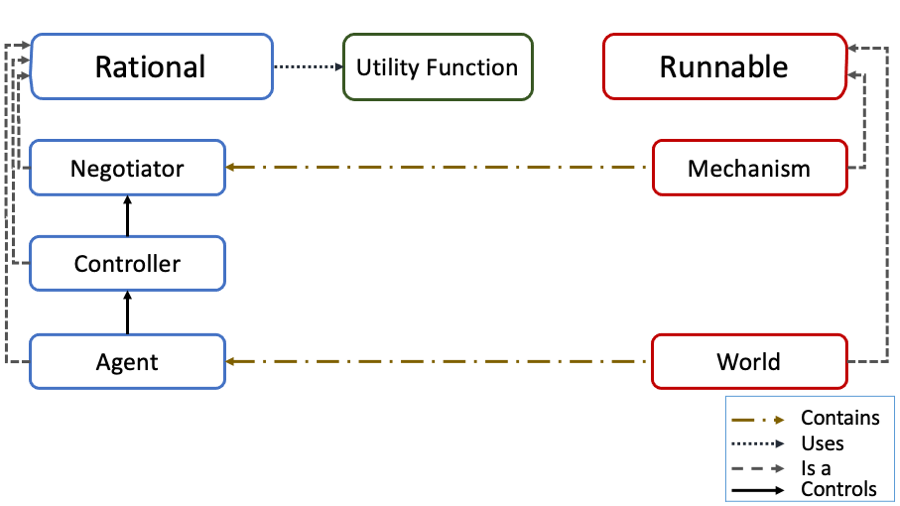
\includegraphics[width=\linewidth]{./figs/agent}
\end{frame}

\begin{frame}[t]
	\frametitle{NegMAS in two slides}
	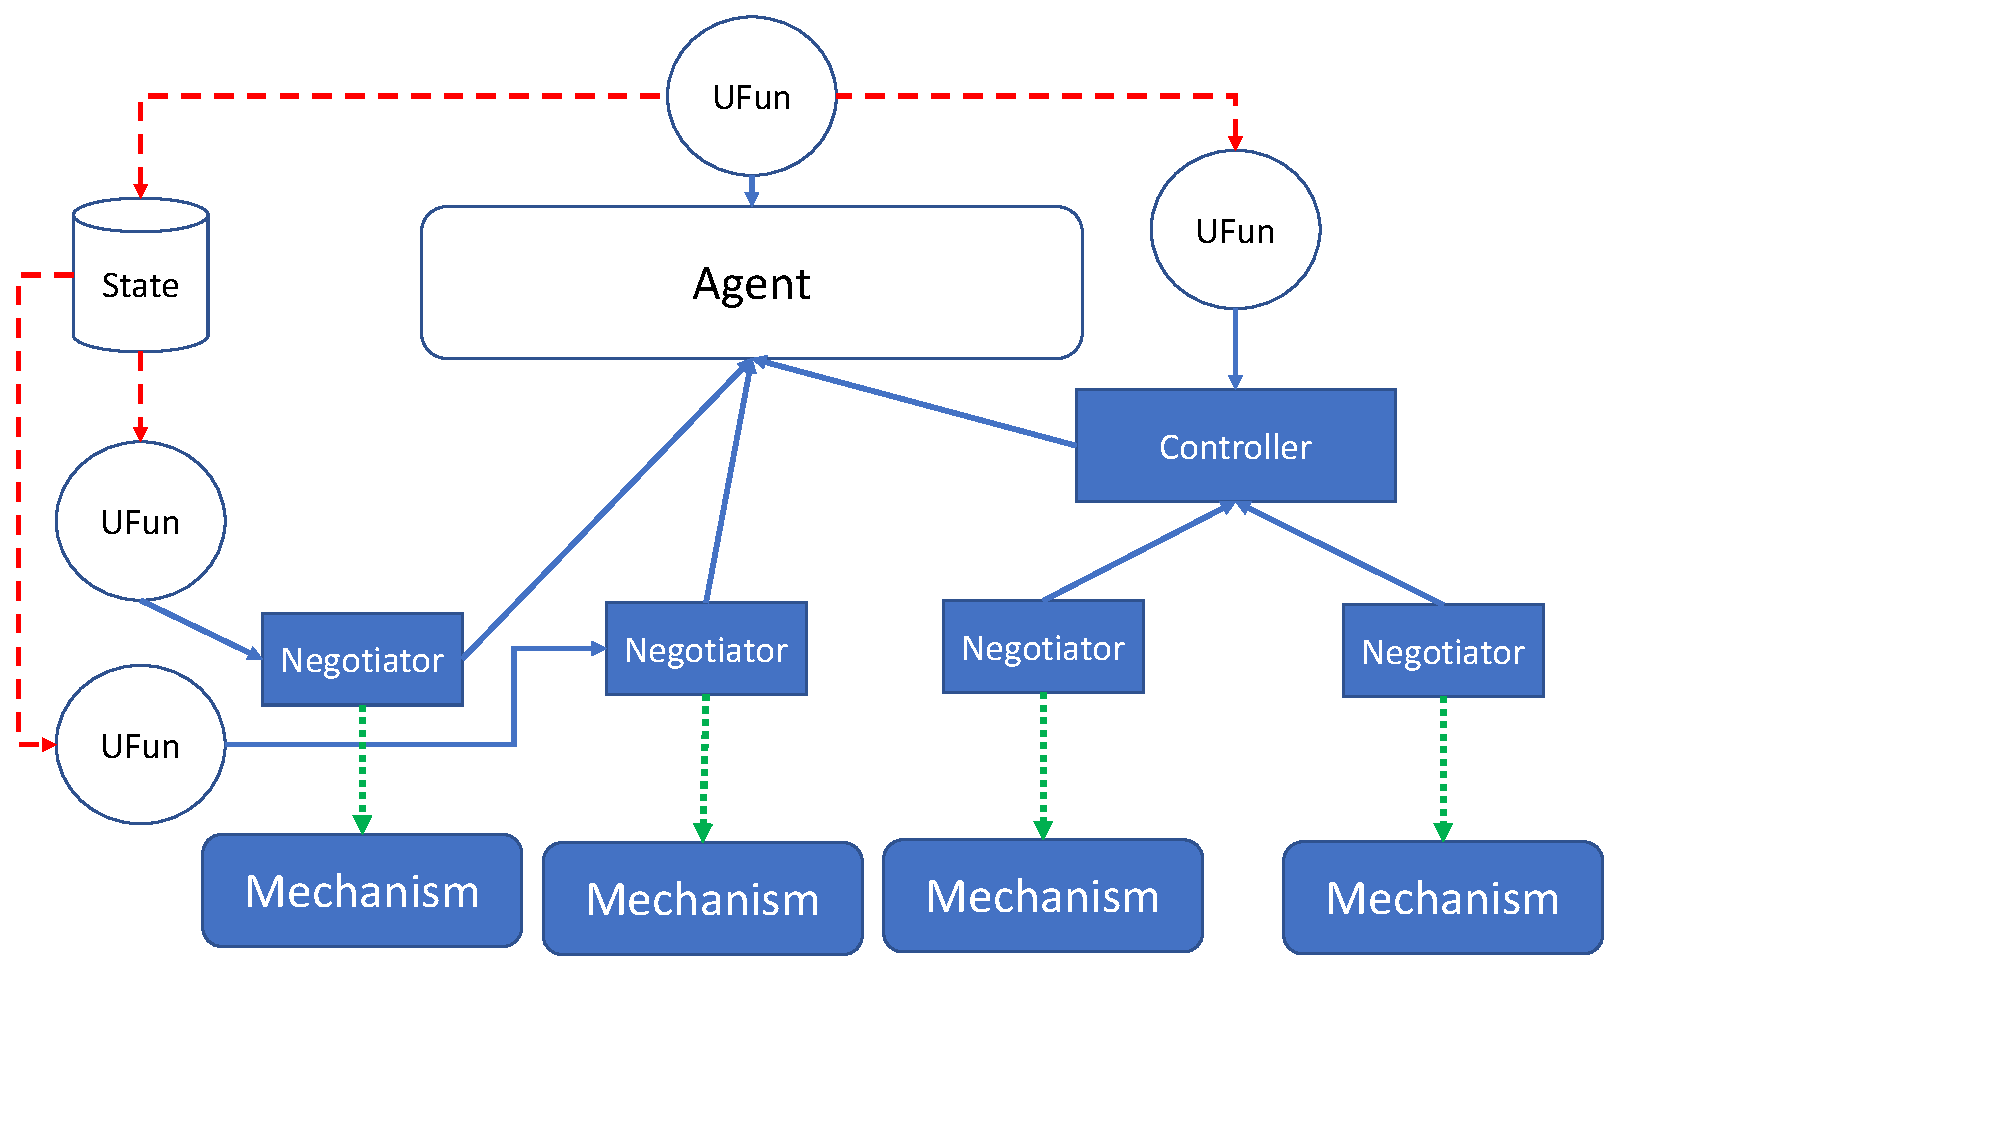
\includegraphics[width=\linewidth]{./figs/negmas_example}
\end{frame}

\begin{frame}[t]
	\frametitle{NegMAS in two slides ( ... OK 3 )}
	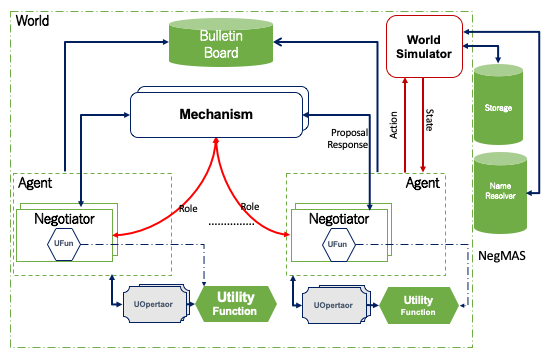
\includegraphics[width=\linewidth]{./figs/world}
\end{frame}

\begin{frame}[t]
	\frametitle{NegMAS in two slides ( ... really!!! )}
	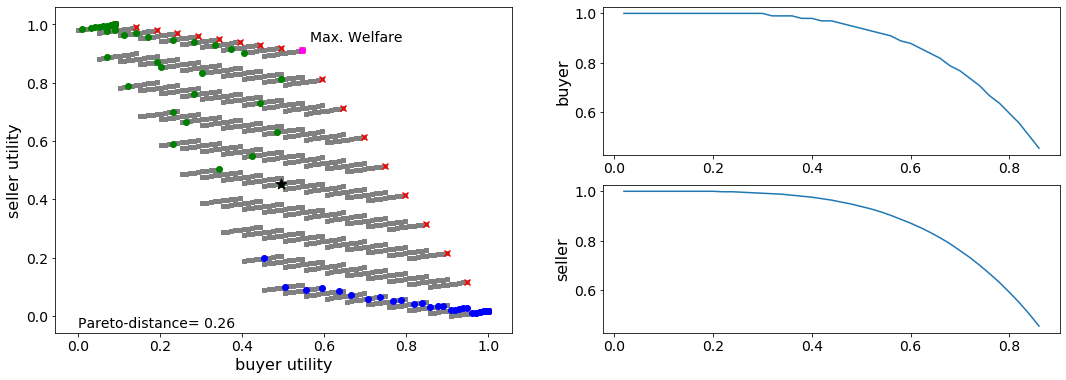
\includegraphics[width=\linewidth]{./figs/negotiation}
	\begin{itemize}
		\item An Example negotiation.
		\item Can you spot a problem?
	\end{itemize}
\end{frame}

\section[SCML]{Automated Negotiation in Supply Chain Management}

\subsection{Motivation}
\begin{frame}[t]
	\frametitle{Negotiation in SCM Business}

	\begin{columns}
		\begin{column}{0.3\textwidth}
			
\includegraphics[width=\linewidth]{./figs/contractroom}
		\end{column}
		\begin{column}{0.4\textwidth}
		\end{column}
		\begin{column}{0.3\textwidth}
			
\includegraphics[width=\linewidth]{./figs/pactum}
		\end{column}
	\end{columns}

	\begin{itemize}
		\item Human negotiations lead to an estimated 17-40\% \emph{value leakage} in some estimates
			\footnote{\small KPMG report: \href{https://bit.ly/3kDRy6I}\href{https://bit.ly/3kDRy6I}}
			\pause
		\item A recent study suggests that at least 15 companies are working in \emph{contracting support systems}
			\footnote{\small Forrester report: \href{https://bit.ly/3nwXEaY}{https://bit.ly/3nwXEaY}}.
			\pause
		\item A recent UNECE UN/CEFACT proposal to standardize negotiation protocols for SCM and other applications
			\footnote{\small UN/CEFACT Project website: \href{https://bit.ly/38LOsLX}{https://bit.ly/38LOsLX}}
			\pause
		\item More to come~\cite{mohammad2019supply}.
	\end{itemize}
\end{frame}

% \begin{frame}[t]
% 	\frametitle{Situated Negotiation}
% 	\foreach \x in {1, ..., 6}{%
% 		\includegraphics<\x>[width=0.9\linewidth, page=\x]{./figs/situated}
% 	}
% \end{frame}
%

\subsection{World Description}

\begin{frame}[t]
	\frametitle{SCML Competition~\cite{mohammad2019supply}}
	\makebox[\textwidth]{
		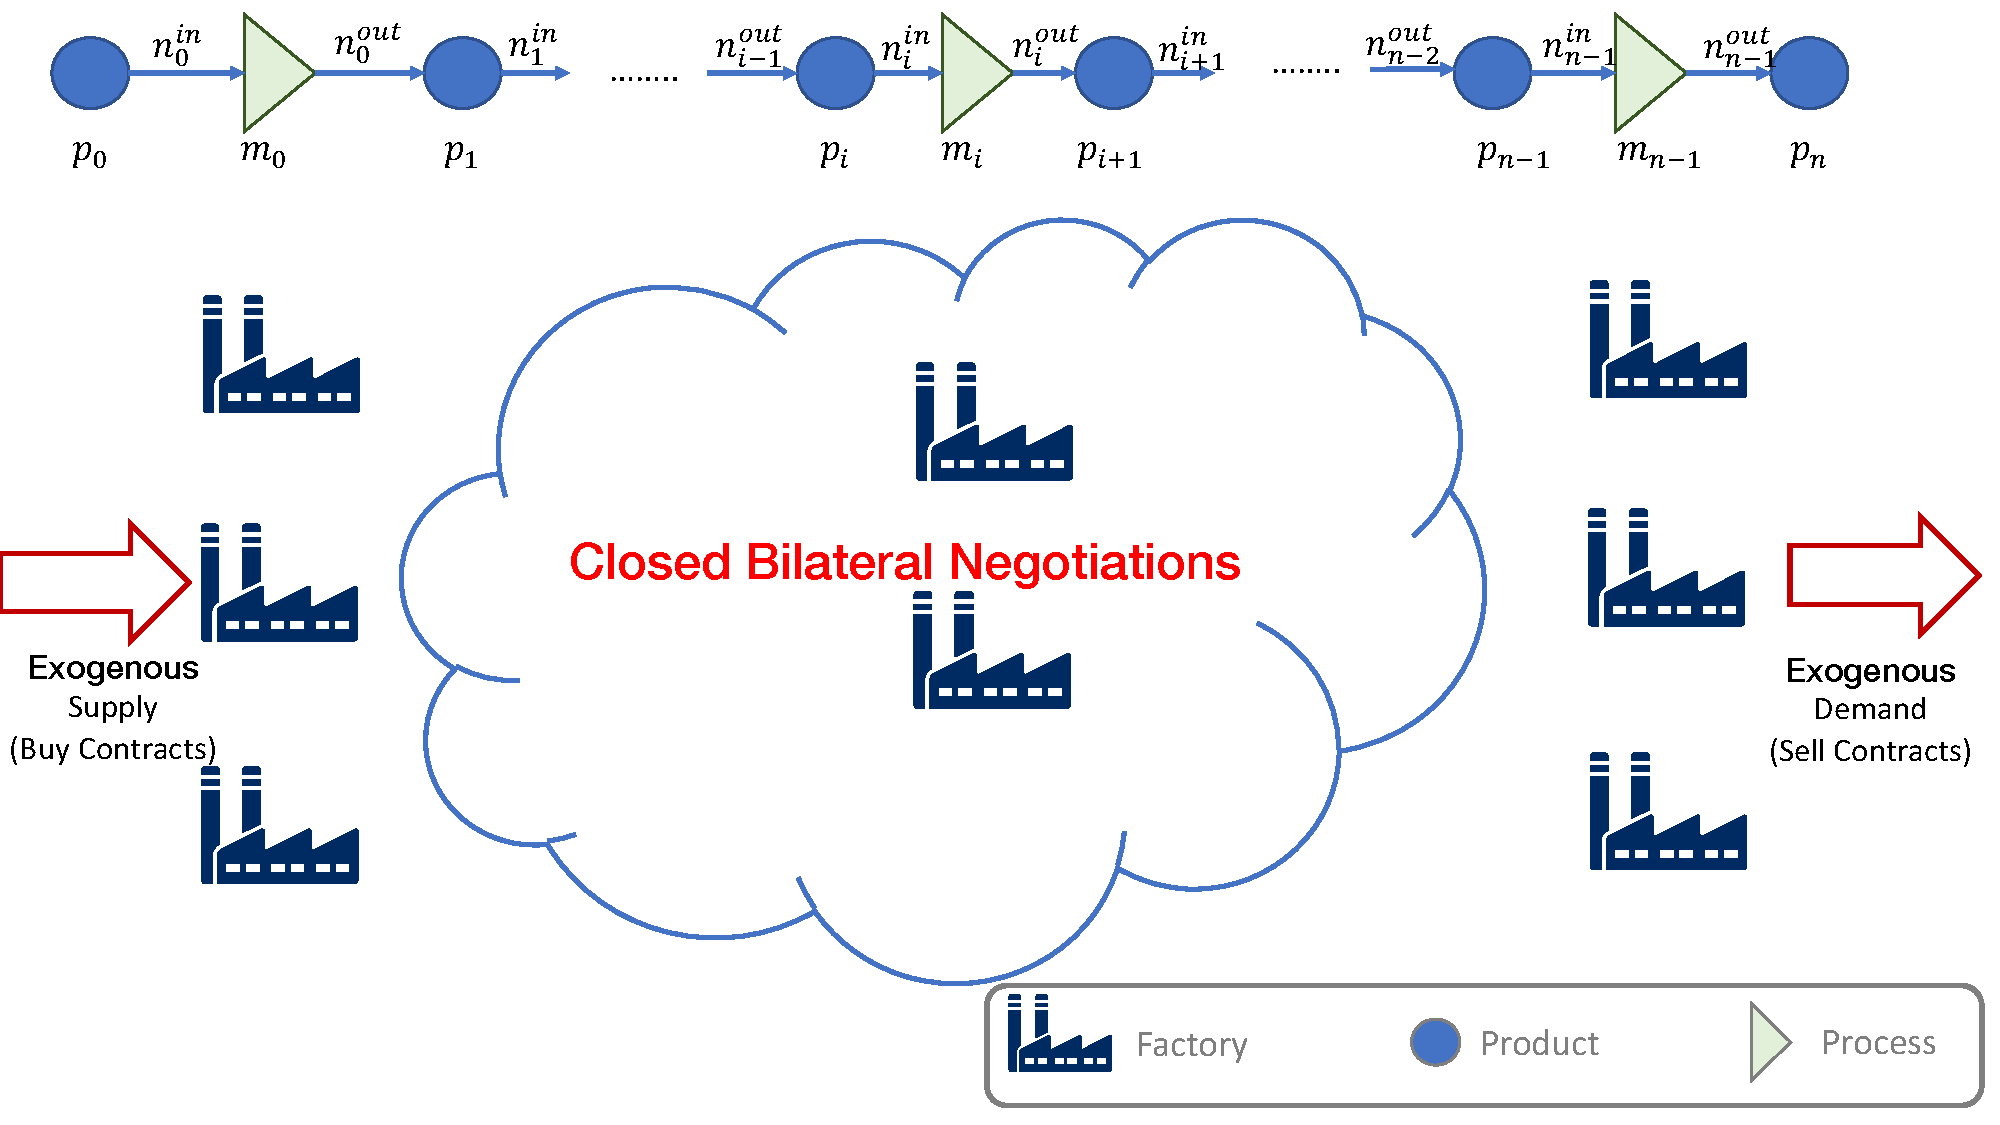
\includegraphics[width=\paperwidth]{./figs/env}
	}
\end{frame}
\begin{frame}[t]
	\frametitle{Example Configuration}
	\makebox[\textwidth]{
		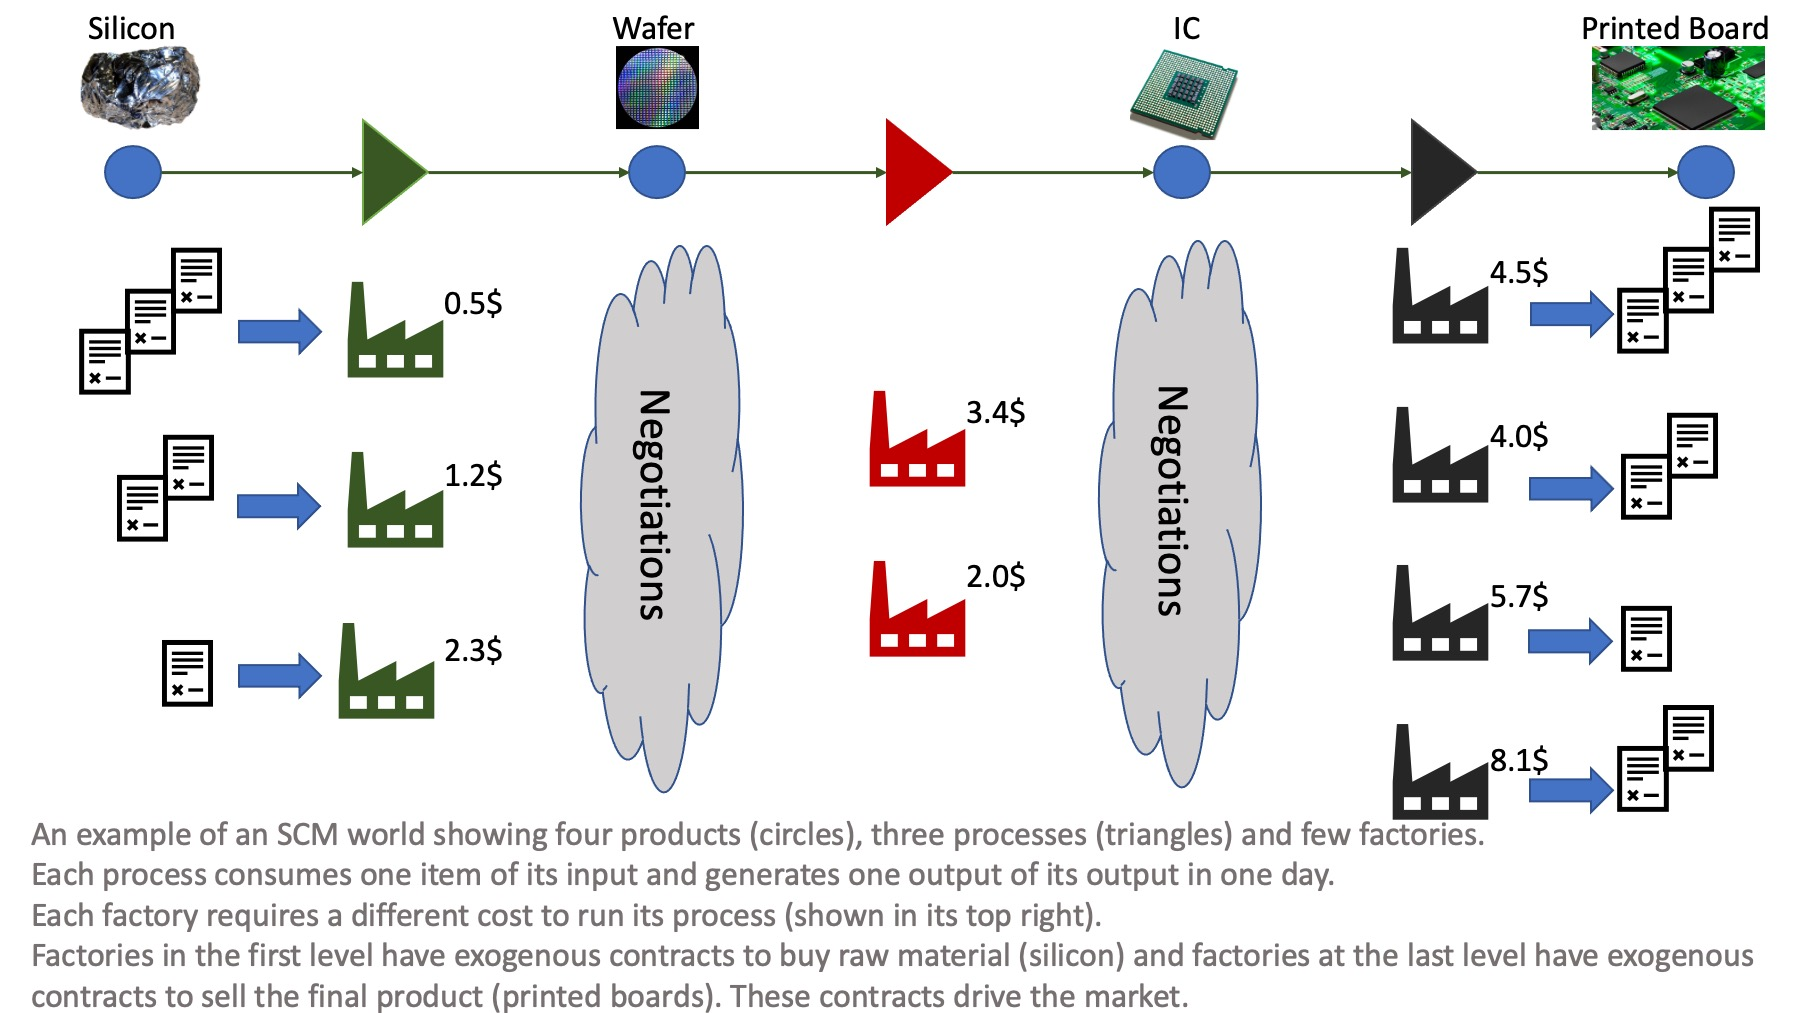
\includegraphics[width=\paperwidth]{./figs/example}
	}
\end{frame}

\begin{frame}[t]
	\frametitle{SCML World}
	\begin{columns}
		\begin{column}{0.5\textwidth}
			\begin{block}{Challenge}
				\begin{itemize}
					\item Turn \textcolor{blue}{maximize profit} into a ufun!!
					\item Dynamic interdependent ufuns.
					\item Sequential negotiations.
					\item Concurrent Negotiations.
					\item Negotiation under uncertainty.
					\item Adaptation and learning.
					\item Trust management.
				\end{itemize}
			\end{block}

			\begin{block}{Information}
				\begin{itemize}
					\item \textbf{Website} \tiny \href{https://scml.cs.brown.edu/}{https://scml.cs.brown.edu/}
					\item \textbf{Code} \tiny \href{GitHub scml}{https://www.github.com/yasserfarouk/scml}
					\item \textbf{Youtube} \tiny \href{https://bit.ly/3pBjZWY}{https://www.youtube.com/playlist?list=PLqvs51K2Mb8IJe5Yz5jmYrRAwvIpGU2nF}
				\end{itemize}
			\end{block}
		\end{column}
		\begin{column}{0.5\textwidth}
			\centering
			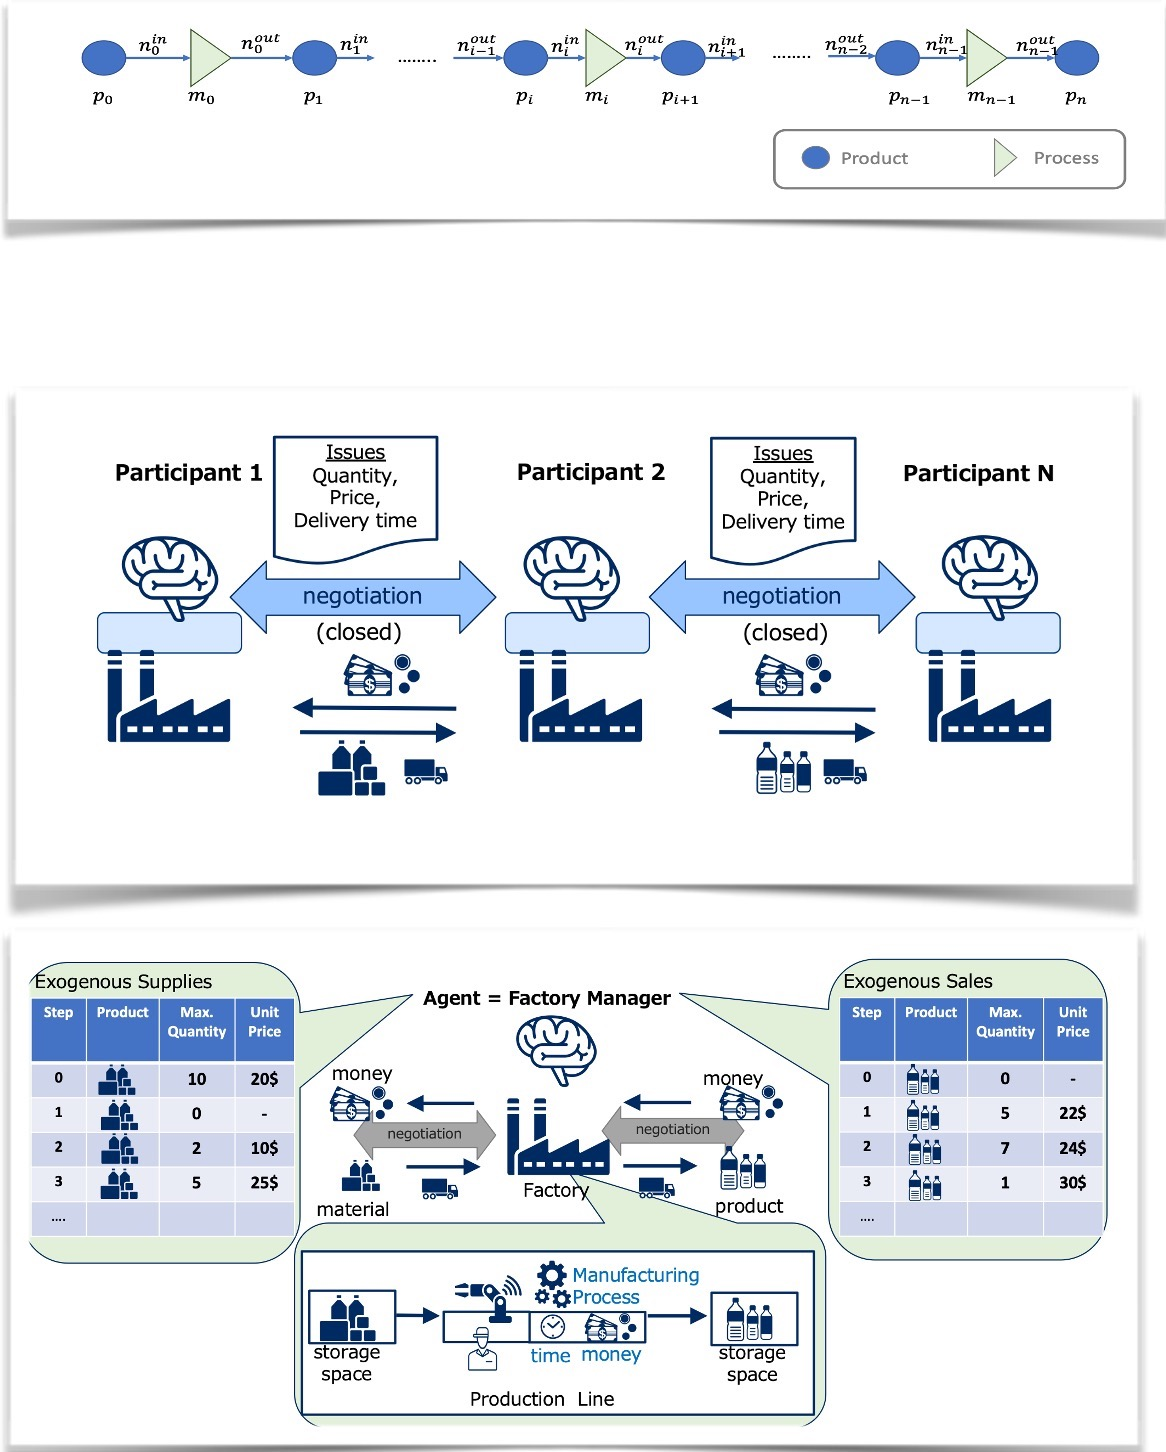
\includegraphics[width=\linewidth]{./figs/sideinfo}
		\end{column}
	\end{columns}
\end{frame}

\begin{frame}[t]
	\frametitle{SCML Competition}
	\begin{columns}
		\begin{column}{0.7\textwidth}
			\begin{block}{Competition Details}
				\begin{itemize}
					\item Runs as part of ANAC \@ IJCAI.
					\item You control one or more factories.
						\begin{itemize}
							\item \textbf{Standard track} $\to$ one factory.
							\item \textbf{Collusion track} $\to$ multiple factories (3).
						\end{itemize}
				\end{itemize}
			\end{block}
			\begin{block}{Score Evaluation}
				\begin{itemize}
					\item \textbf{Per instantiation}: Total profit counting
						inventory at \blue{half} the \blue{trading} price.
					\item \textbf{Total}: \blue{median} of per-instantiation scores.
				\end{itemize}
			\end{block}
		\end{column}
		\begin{column}{0.3\textwidth}
			\centering
			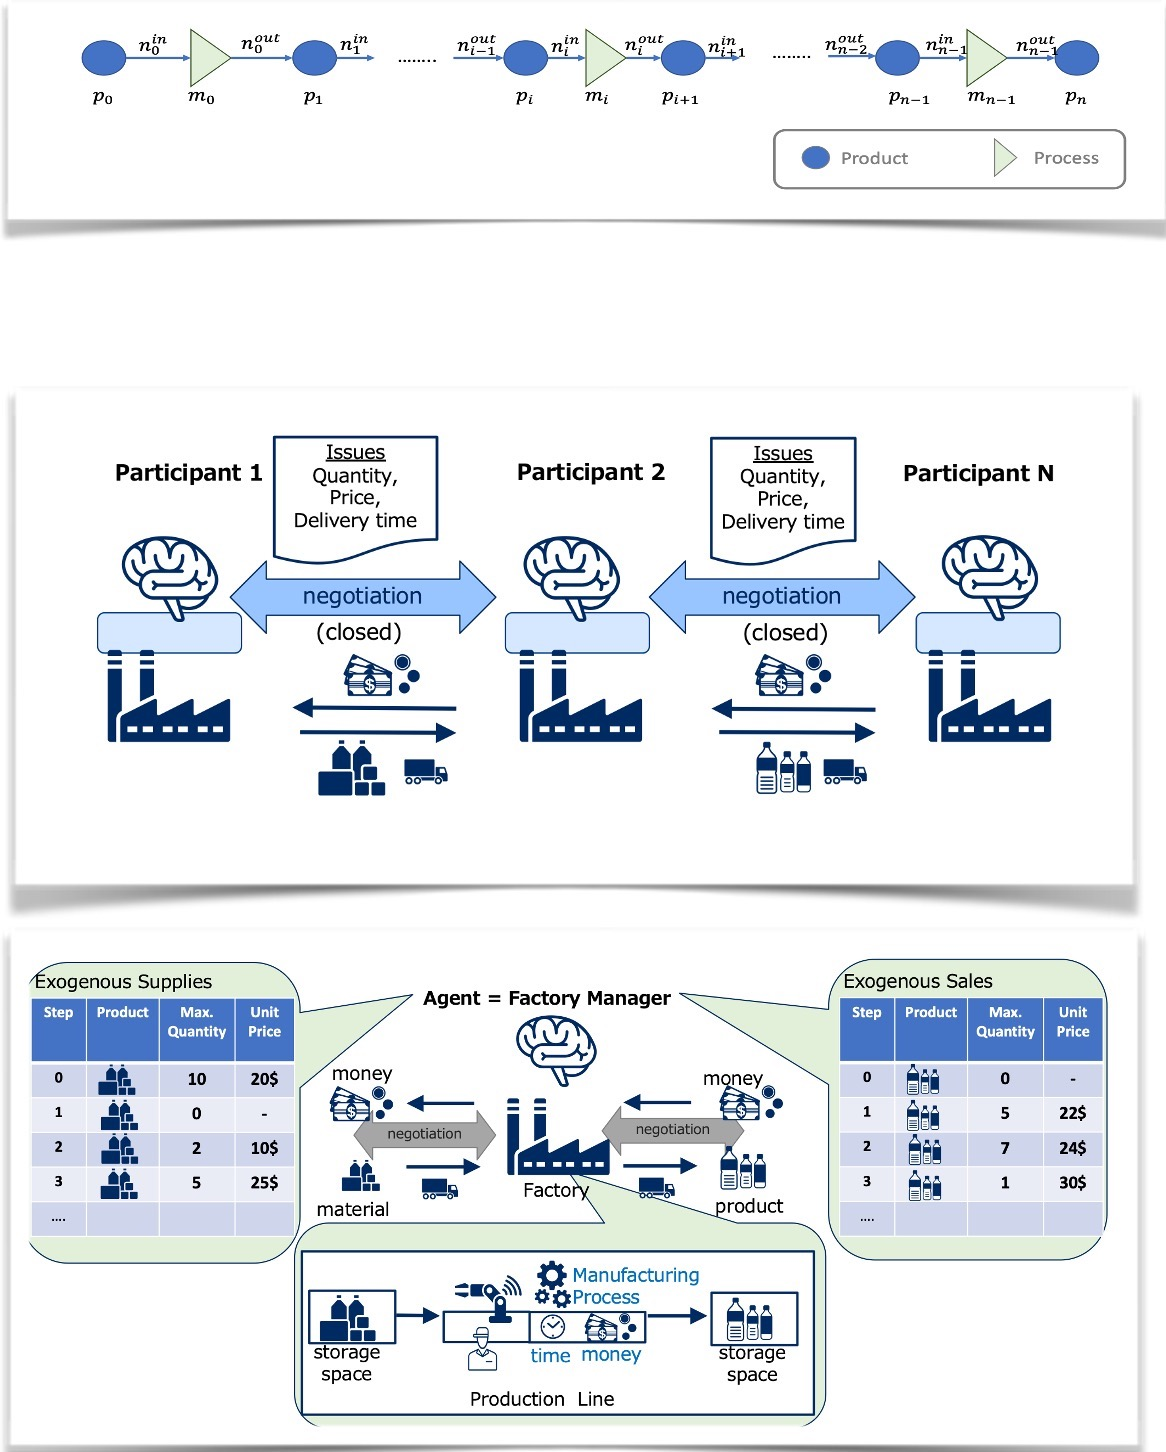
\includegraphics[width=\linewidth]{./figs/sideinfo}
		\end{column}
	\end{columns}
\end{frame}

\begin{frame}[t]
	\frametitle{Simulation Steps}
	\begin{adjustwidth}{-2.5em}{0em}
		% \begin{overprint}
		% 	\makebox[\textwidth]{
		\foreach \x in {1, ..., 8}{
			\includegraphics<\x>[width=\paperwidth, page=\x]{./figs/steps}
		}
		% 	}
		% \end{overprint}
	\end{adjustwidth}
\end{frame}

\begin{frame}[t]
	\frametitle{Trading prices}
	\centering
	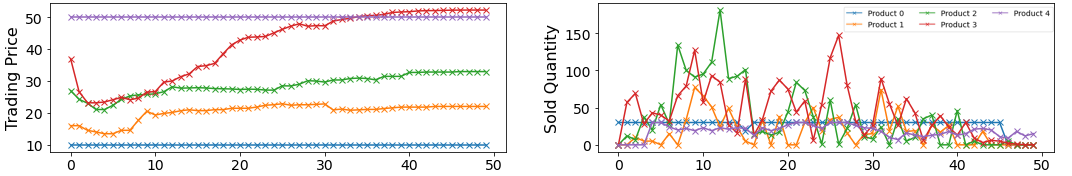
\includegraphics[width=\linewidth]{figs/trading.png}
	\begin{block}{What is trading price and why is it calculated?}
		\begin{itemize}
			\item A value calculated by the system \blue{for each product}.
			\item Represents some estimate of the \blue{current} price.
			\item \blue{Never revealed} to agents.
			\item Usages:
				\begin{itemize}
					\item Used at the end to value inventory.
					\item Used when calculating \blue{spot-market price}.
						during breach processing.
				\end{itemize}
		\end{itemize}
	\end{block}
	\begin{block}{How does the system calculate it?}
		\[
			\tp (p, s) =
			\frac{\beta^{s+1} \; Q_{-1}(p) \; \cat (p) + \sum_{i=0}^{s}
				\beta^{s-i} \; Q_{i} (p) \; \mu_i (p)}{\beta^{s+1}+\sum_{i=0 \mid
			Q_{i}(p)>0}^{s} \beta^{s-i}} \enspace ,
		\]
	\end{block}
\end{frame}
\begin{frame}[t]
	\frametitle{Trading prices: The details}
	\begin{block}{Quantities and prices}
		\[
			Q_i (p') = \sum_{\{c \in C^i \mid c.p = p' \}} c.\bar q
		\]
		\[
			\mu_i (p') = \frac{\sum_{\{c \in C^i \mid c.p = p'\}} c.\bar q \times c.u}{Q_i (p')}
		\]
	\end{block}

	\begin{block}{How does the system calculate it?}
		\[
			\tp (p, s) =
			\frac{\beta^{s+1} \; Q_{-1}(p) \; \cat (p) + \sum_{i=0}^{s}
				\beta^{s-i} \; Q_{i} (p) \; \mu_i (p)}{\beta^{s+1}+\sum_{i=0 \mid
			Q_{i}(p)>0}^{s} \beta^{s-i}} \enspace ,
		\]
	\end{block}
\end{frame}
\begin{frame}[t]
	\frametitle{When things go wrong}
	\begin{columns}
		\begin{column}{0.6\textwidth}
			\begin{block}{What is a breach}
				\begin{itemize}
					\item Insufficient funds or insufficient inventory.
				\end{itemize}
			\end{block}
			\begin{block}<2->{Breach Processing}
				\begin{itemize}[<+->]
					\item A breach report is \textbf{always} published.
						\begin{itemize}
							\item who and fraction.
						\end{itemize}
					\item Insufficient products $\to$ \textbf{forced to} buy
						from the \blue{spot market}.
					\item Insufficient funds $\to$ bankruptcy.
						\begin{itemize}
							\item bankruptcy $\to$ liquidation.
						\end{itemize}
				\end{itemize}
			\end{block}
		\end{column}
		\begin{column}{0.4\textwidth}
			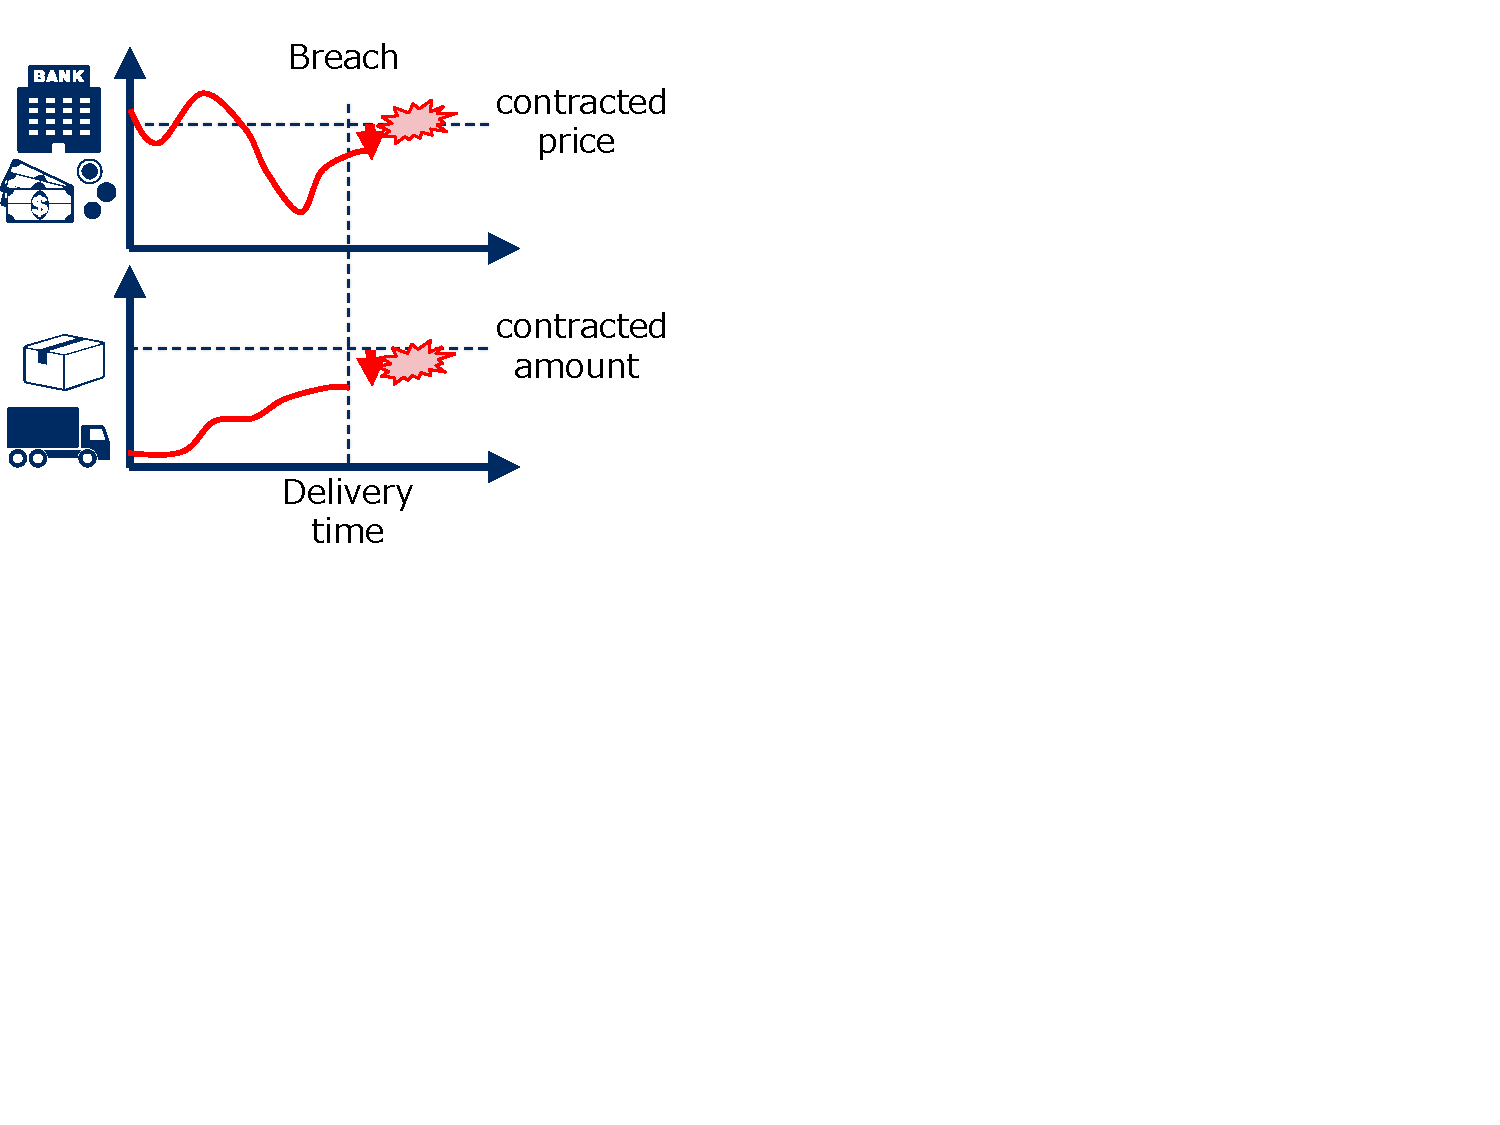
\includegraphics[width=\linewidth]{figs/breach.pdf}
		\end{column}
	\end{columns}
\end{frame}

\begin{frame}[t]
	\frametitle{Spot Market}
	\begin{block}{Spot market}
		\begin{itemize}[<+->]
			\item \textbf{No-choice:} Can be used \textbf{only} for insufficient inventory
				breaches.
			\item \textbf{Penalizing:} Entails higher price than the \blue{trading price}
			\item \textbf{Personalized:} More breaches $\to$ higher spot price
				\textbf{for you}
		\end{itemize}
	\end{block}
	\begin{block}{Calculation}
		\begin{itemize}[<+->]
			\item Agent's spot price penalty:
				\(
				\sm_a (p, s) = \lambda \sum_{i=0}^{s} {\alpha^{s-i} q_a (p, i)} \enspace,
				\)
			\item Breaching agents buy \textbf{expensive}:
				\[\tp(p, s) \times (1+\gl) \times (1+\sm_a(p,s))\]
			\item Bankrupt agents are liquidated \textbf{cheap}:
				\[\tp(p, s) / ((1+\gl) \times (1+\sm_a(p,s))\]
		\end{itemize}
	\end{block}
\end{frame}

\begin{frame}[t]
	\frametitle{Bankruptcy Processing}
	\begin{block}{Bankruptcy conditions}
		\begin{itemize}[<+->]
			\item Insufficient money for a buy contract.
			\item Insufficient money to buy from the spot market for
				as sell contract.
		\end{itemize}
	\end{block}
	\begin{block}{What exactly happens?}
		\begin{enumerate}[<+->]
			\item The agent is stopped from every buying or selling.
			\item Its inventory is sold on the spot market.
			\item All agents are informed.
			\item Agents with future contracts with it are
				informed about the expected level of breach.
			\item The agent's score is set to $-1$.
		\end{enumerate}
	\end{block}
\end{frame}
\begin{frame}[t]
	\frametitle{When things go wrong: Summary}
	\begin{columns}
		\begin{column}{0.5\textwidth}
			\begin{block}{Summary}
				\begin{itemize}[<+->]
					\item An unfulfilled contract is reported to the
						\textbf{breach-list} (who and fraction).
					\item Insufficient funds $\to$ bankrupt.
						\item Insufficient product $\to$ buy at high
							cost.
							\begin{itemize}
								\item Cannot buy $\to$ bankrupt.
							\end{itemize}
						\item Bankrupt $\to$ \textbf{really really bad}
							\begin{itemize}
								\item No more trade.
								\item Very low score.
								\item All inventory is liquidated.
								\item May hurt other agents.
							\end{itemize}
				\end{itemize}
			\end{block}
		\end{column}
		\begin{column}{0.5\textwidth}
			\includegraphics<1->[width=\textwidth]{figs/breach.pdf}
		\end{column}
	\end{columns}
\end{frame}

\section{Agent}
\begin{frame}[t]
	\frametitle{Agent Knowledge}
	\begin{block}{About itself}
		\begin{itemize}
			\item \textbf{Its capabilities:} lines and production cost.
			\item \textbf{Its location:} input and output products.
			\item \textbf{Its partners:} suppliers and consumers (and competitors).
			\item \textbf{Its state:} inventory, wallet, contracts, and negotiations.
		\end{itemize}
	\end{block}
	\pause
	\begin{block}{About the market}
		\begin{itemize}
			\item The production graph and factories at each level.
			\item Time and simulation length.
		\end{itemize}
	\end{block}
	\pause
	\begin{block}{About others}
		\begin{itemize}
			\item \textbf{Financial Reports:} balance, assets,
				breach fraction/probability.
			\item \textbf{Past Interactions:} negotiations and
				contracts between itself and that agent.
		\end{itemize}
	\end{block}
\end{frame}
\begin{frame}[t]
	\frametitle{Development Approaches}
	\begin{block}{Monolithic Agent}
		\begin{itemize}
			\item Respond to callbacks in the \textcolor{blue}{Agent} class.
			\item Functionality is distributed \textbf{among callbacks}.
			\item Everything is in one place (the agent class).
			\item Harder to reuse.
		\end{itemize}
	\end{block}

	\begin{block}{Component-Based Agent}
		\begin{columns}
			\begin{column}{0.5\textwidth}

				\begin{itemize}
					\item Divides the agent into \textcolor{blue}{semi-independent} components.
					\item Functionality is distributed between \textbf{components}.
					\item Easier to reuse.
				\end{itemize}
			\end{column}
			\begin{column}{0.5\textwidth}
				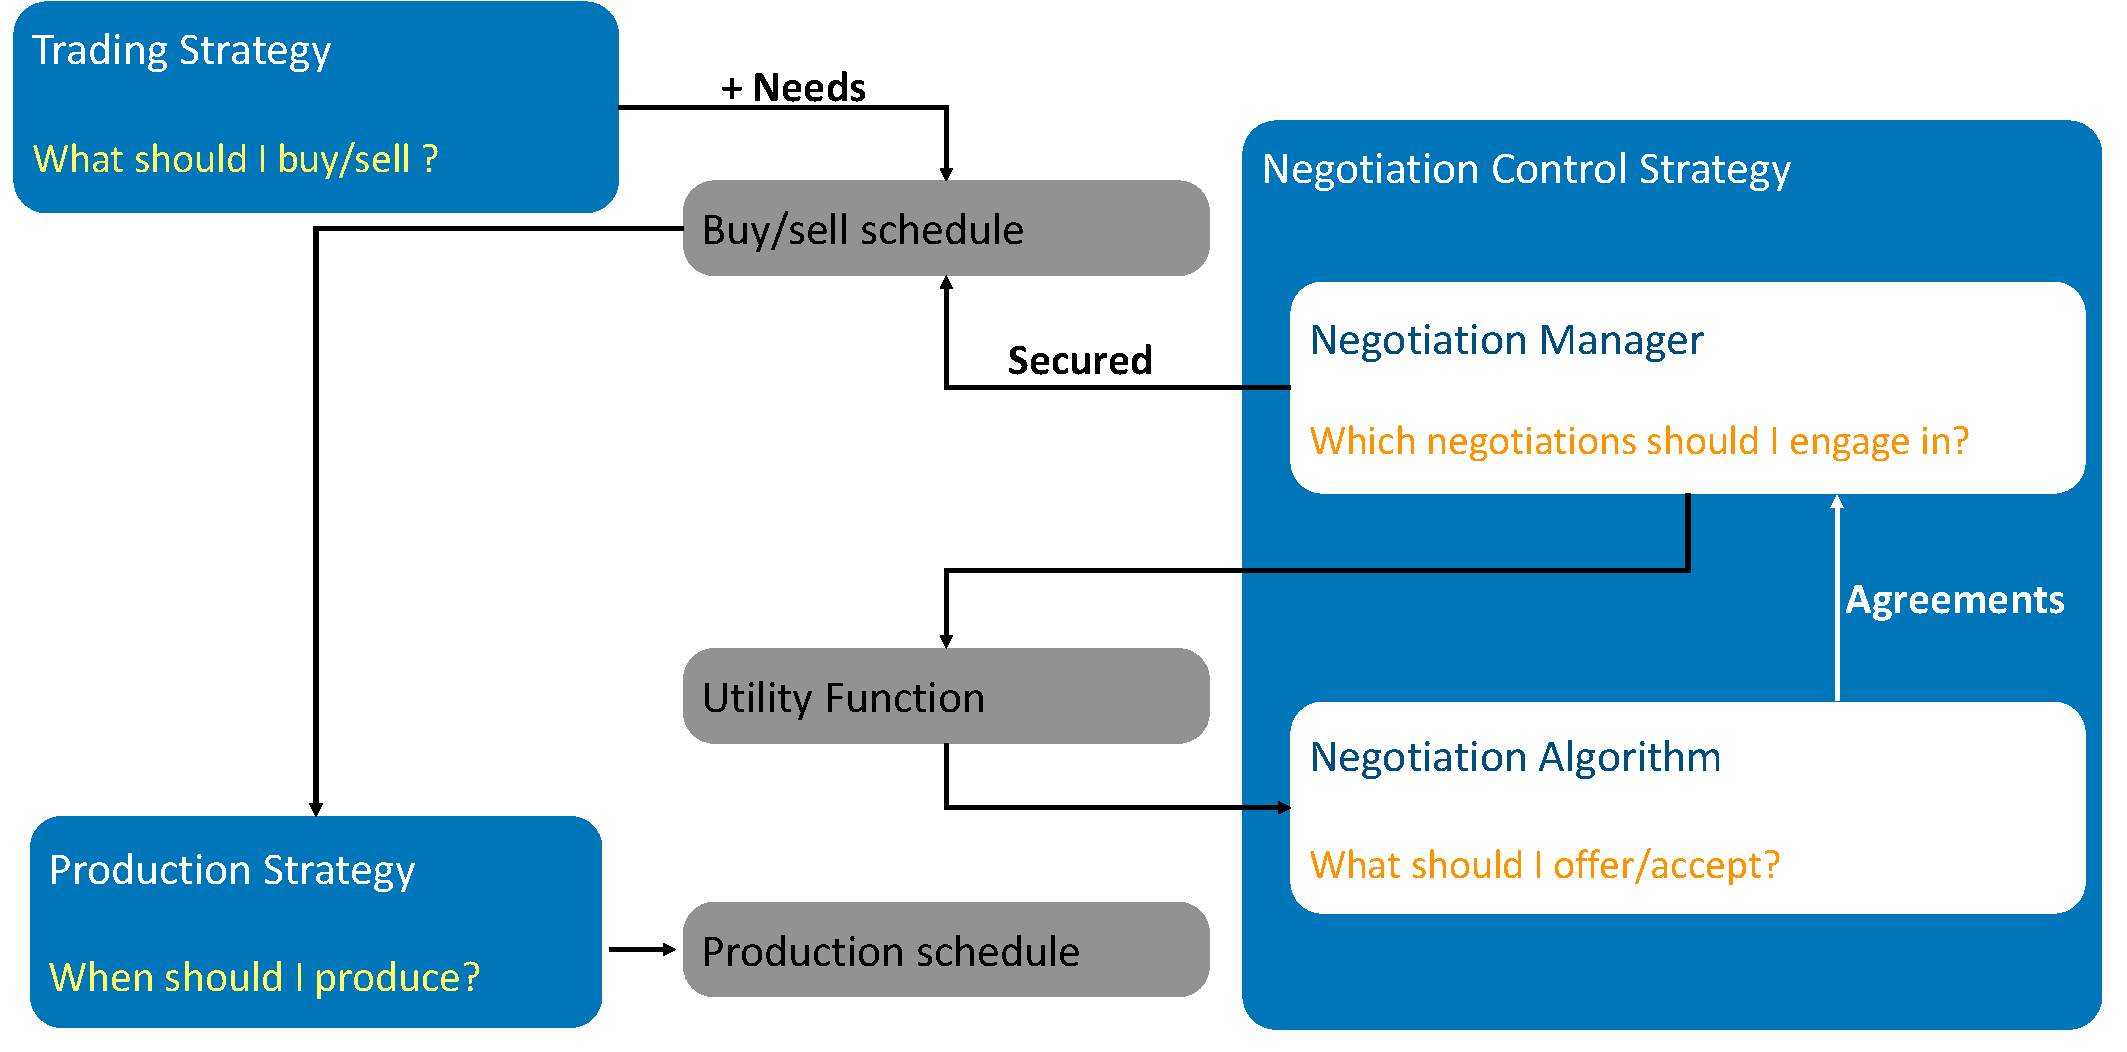
\includegraphics[width=0.95\textwidth]{./figs/cba}
			\end{column}
		\end{columns}
	\end{block}
\end{frame}

\begin{frame}[t]
	\frametitle{Callbacks and Timing}
	\begin{adjustwidth}{-2.5em}{0em}
		% \begin{overlayarea}{\textwidth}{\textheight}
		% 	\begin{figure}
		% 		\centering
		% \makebox[\textwidth]{
		\foreach \x in {1, ..., 18}{
			\includegraphics<\x>[width=\paperwidth, page=\x]{./figs/callbacks}
		}
		% 	}
		% \end{figure}
		% \end{overlayarea}
	\end{adjustwidth}
\end{frame}
\begin{frame}[t]
	\frametitle{What is a component?}
	\begin{adjustwidth}{-2.5em}{0em}
		\foreach \x in {1, ..., 8}{
			\includegraphics<\x>[width=\paperwidth, page=\x]{./figs/component.pdf}
		}
	\end{adjustwidth}
\end{frame}

\begin{frame}[t]
	\frametitle{SCML Agent Components}
	\begin{adjustwidth}{-2.5em}{0em}
		\foreach \x in {1, ..., 9}{
			\includegraphics<\x>[width=\paperwidth, page=\x]{./figs/component_details.pdf}
		}
	\end{adjustwidth}
\end{frame}

\begin{frame}[t]
	\frametitle{Trading Strategy}
	\begin{exampleblock}{Role}
		\begin{columns}
			\begin{column}{0.35\textwidth}
				
\includegraphics[width=\linewidth]{./figs/orchestrating.jpeg}
			\end{column}
			\begin{column}{0.6\textwidth}
				\begin{itemize}
					\item Decides an overall \textbf{business plan}.
					\item Keeps track of buy/sell \textbf{needs}.
				\end{itemize}
			\end{column}
		\end{columns}
	\end{exampleblock}
	\begin{block}{Built-in Options}
		\begin{description}
			\item[No Strategy] yes, just do nothing.
			\item[Reactive] Zero needs.
			\item[Prediction Based] trade and execution prediction.
				\begin{itemize}
					\item Needs come from trade predictions.
					\item Secured inputs/outputs come from execution prediction.
				\end{itemize}
		\end{description}
	\end{block}
\end{frame}

\begin{frame}[t]
	\frametitle{Negotiation Manager}
	\begin{exampleblock}{Role}
		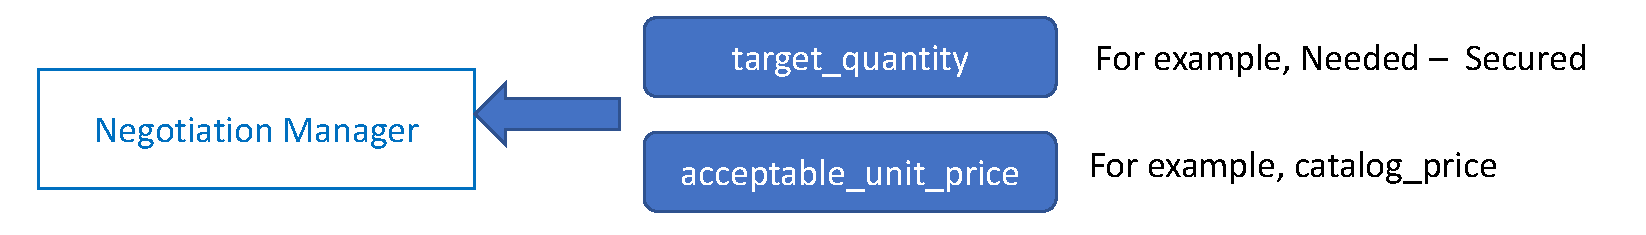
\includegraphics[width=\linewidth]{./figs/negmanager}
		Controls negotiation.
		\begin{itemize}
			\item Sets negotiation agendas $\to$ \textbf{ Proactive }.
			\item Accepts/rejects negotiation requests $\to$ \textbf{ Reactive }.
			\item Defines utility functions.
			\item Goal: Achieve the target put by the trading strategy.
		\end{itemize}
	\end{exampleblock}
	\begin{block}{Built-in Options}
		\begin{description}
			\item[Independent Negotiations] buy cheap ASAP, sell expensive ALAP.
			\item[Moving Range] Creates one controller for selling and another for buying.
			\item[Step Manager] Creates one controller per simulation step.
		\end{description}
	\end{block}
\end{frame}

\begin{frame}[t]
	\frametitle{Production Strategy}
	\begin{exampleblock}{Role}
		\centering
		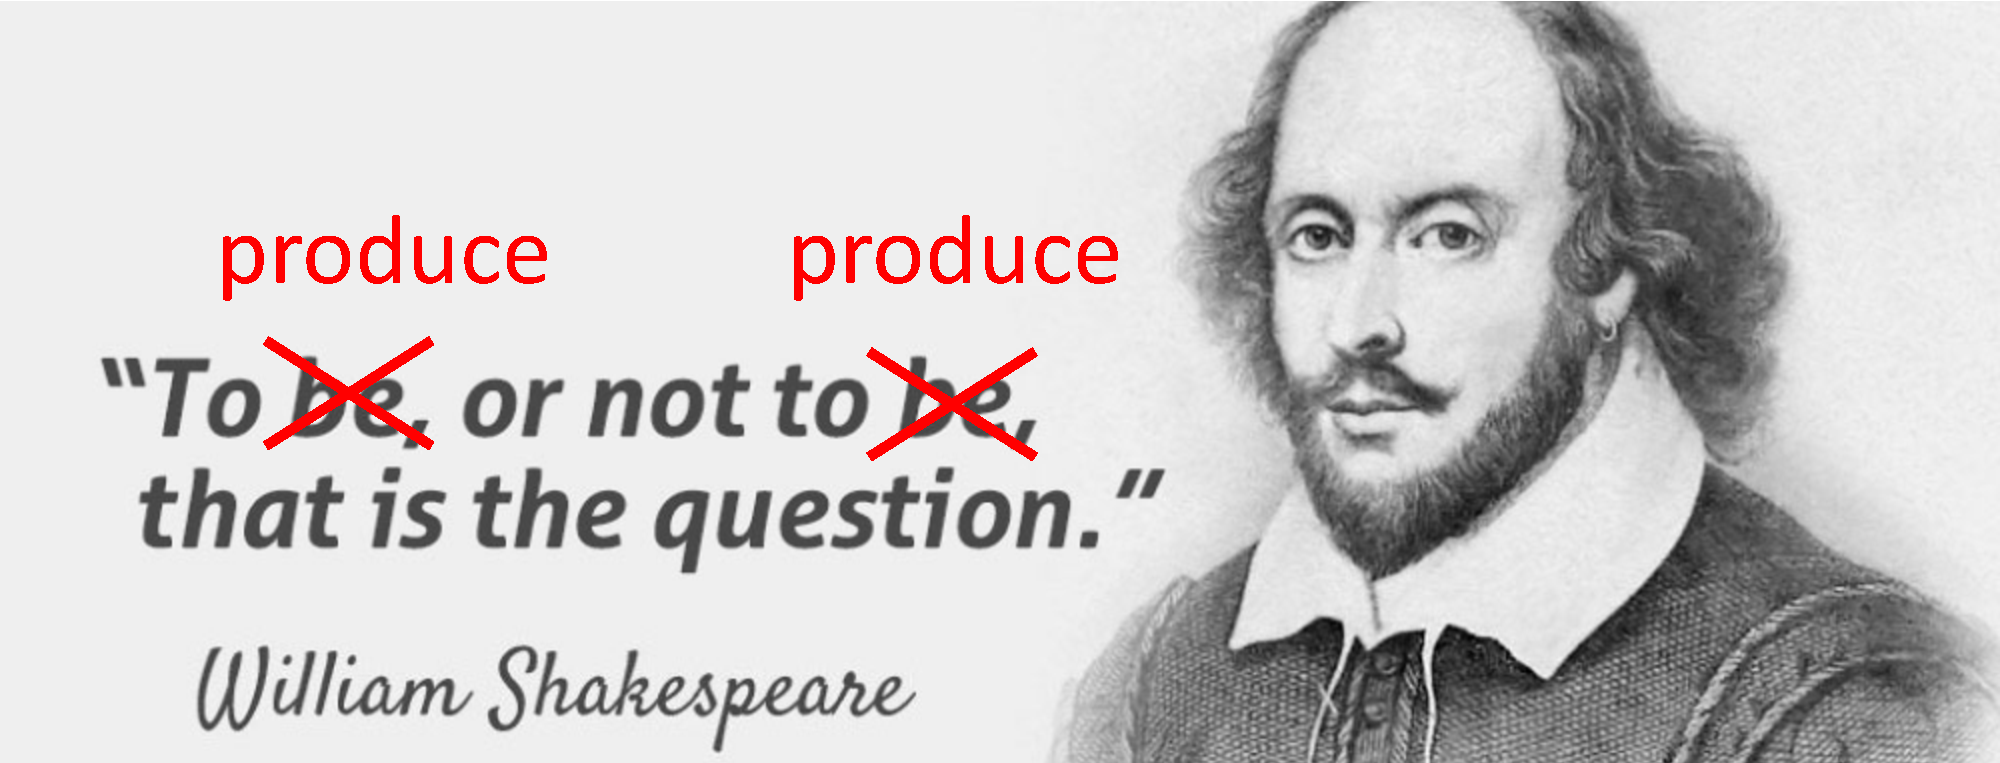
\includegraphics[width=0.6\linewidth]{./figs/toproduce}
	\end{exampleblock}
	\begin{block}{Built-in Options}
		\begin{description}
			\item[Supply Driven] Produce based on \textbf{buy} contracts.
				\begin{itemize}
					\item Inventory is always valued at the end.
				\end{itemize}
			\item[Demand Driven] Produce based on \textbf{sell} contracts.
				\begin{itemize}
					\item ... but inventory is valued at half the \emph{trading} price!
				\end{itemize}
		\end{description}
	\end{block}
\end{frame}
% \section{Development Environment}
% \subsection{Installation}
% \subsection{Simulation}
% \subsection{Tournament}
% \section{Live Demo}
% \subsection{An ML Based Trading Strategy}
% \subsection{A complete Agent}
% \section{Development Examples}
% \subsection{MontyHall}
% \subsection{Merchant}
% \subsection{Agent30}
\section{Conclusion}

% \begin{frame}{Conclusion}
% 	\begin{columns}
% 		\begin{column}{0.7\textwidth}
% 			\setbeamercovered{transparent}
% 		\end{column}
% 		\begin{column}{0.3\textwidth}
% 			\includegraphics<1->[width=1\textwidth]{figs/unmediated}
% 			\includegraphics<1->[width=1\textwidth]{figs/session}
% 			\includegraphics<1->[width=1\textwidth]{figs/aspiration}
% 		\end{column}
% 	\end{columns}
% 	\pause
% 	\begin{exampleblock}{}
% 		\centering
% 		Thank you for listening (y.mohammad@aist.go.jp)
% 	\end{exampleblock}
% \end{frame}

\begin{frame}[t]
	\frametitle{Summary}
	\begin{columns}
		\begin{column}{0.5\textwidth}
			\begin{block}{Challenge}
				\begin{itemize}
					\item Turn \textcolor{blue}{maximize profit} into a ufun!!
					\item Dynamic interdependent ufuns.
					\item Sequential negotiations.
					\item Concurrent Negotiations.
					\item Negotiation under uncertainty.
					\item Adaptation and learning.
					\item Trust management.
				\end{itemize}
			\end{block}

			\begin{block}{Information}
				\begin{itemize}
					\item \textbf{Website} \tiny \href{https://scml.cs.brown.edu/}{https://scml.cs.brown.edu/}
					\item \textbf{Code} \tiny \href{GitHub scml}{https://www.github.com/yasserfarouk/scml}
					\item \textbf{Youtube} \tiny \href{https://bit.ly/3pBjZWY}{https://www.youtube.com/playlist?list=PLqvs51K2Mb8IJe5Yz5jmYrRAwvIpGU2nF}
				\end{itemize}
			\end{block}
		\end{column}
		\begin{column}{0.5\textwidth}
			\centering
			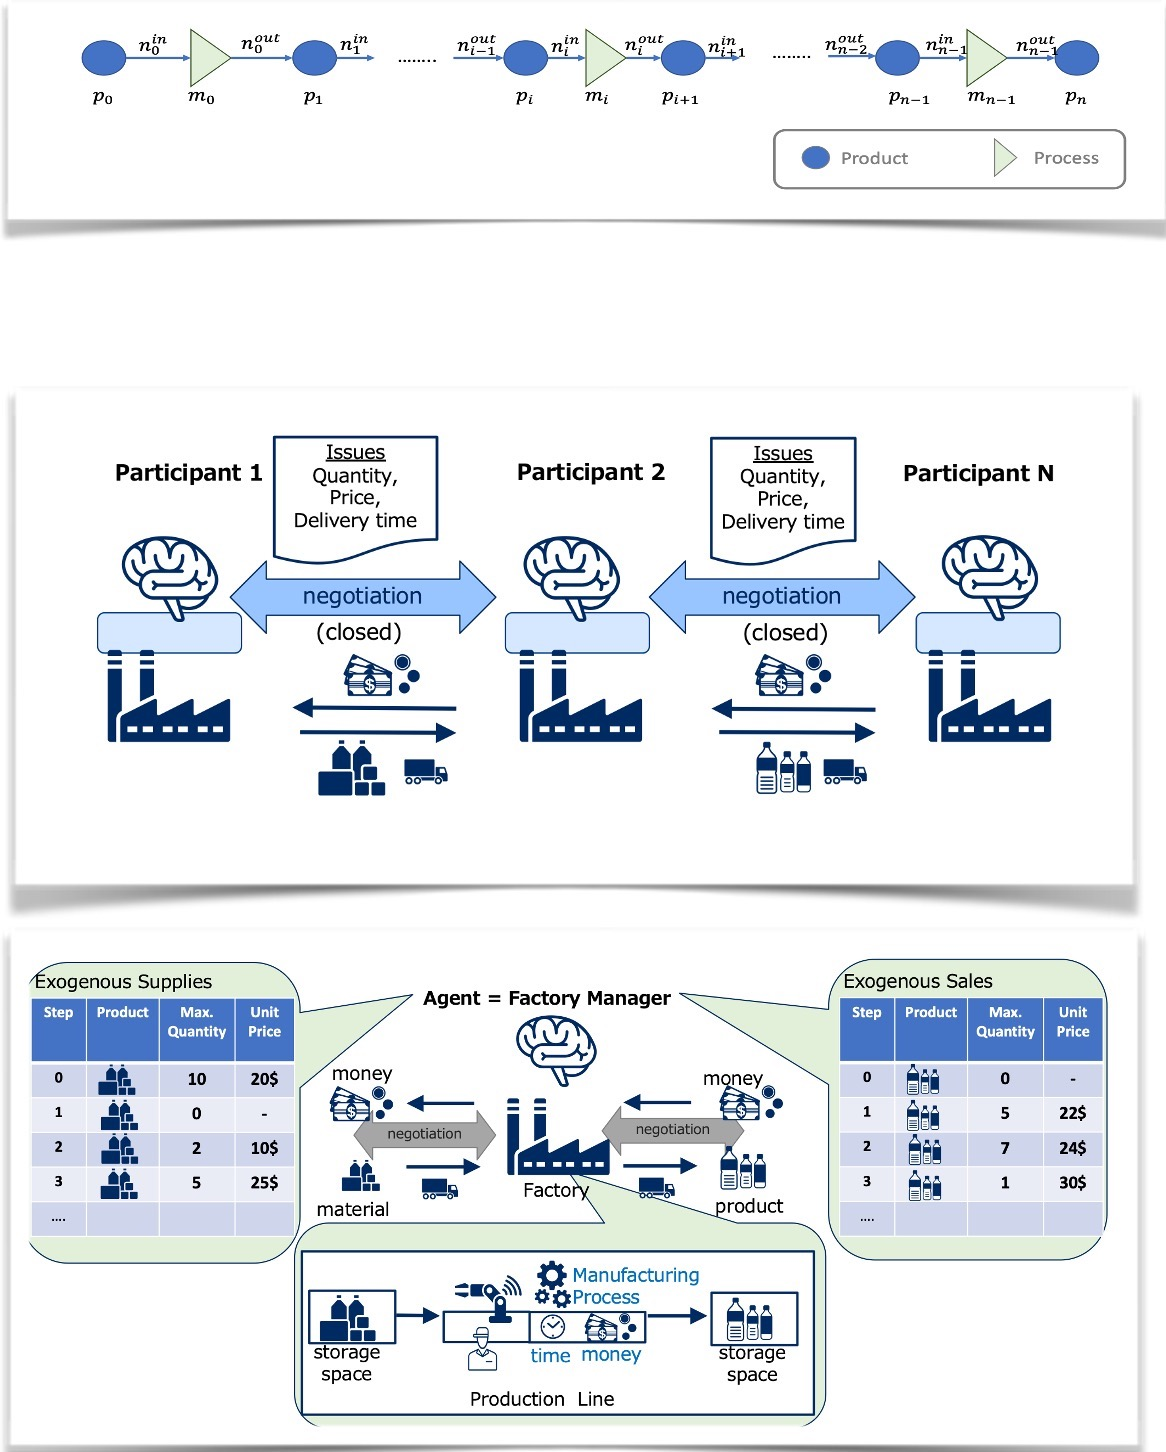
\includegraphics[width=\linewidth]{./figs/sideinfo}
		\end{column}
	\end{columns}
\end{frame}
\begin{frame}[allowframebreaks]%in case more than 1 slide needed
	\frametitle{References}
	{\footnotesize
		\bibliographystyle{apalike}
		\bibliography{prima2020_scml_tutorial}
	}
\end{frame}

\end{document}